\documentclass{article}
\usepackage[a4paper, total={6.5in,8.5in}]{geometry}

\usepackage{subcaption}
\usepackage{graphicx}
\usepackage{algorithm}
\usepackage{algpseudocode}
\usepackage{booktabs} 
\usepackage{multirow} 
\usepackage[numbers, sort, comma, square]{natbib}
\usepackage{authblk}
\usepackage{wrapfig}
\usepackage{subcaption}
\usepackage{multicol}
\usepackage{array}
\usepackage{float}
\usepackage{hyperref}
\usepackage{booktabs}
\usepackage{siunitx}
\usepackage{subcaption}
\usepackage{rotating}
\usepackage{caption}
\usepackage{amsmath,amsfonts,bm}
\usepackage{amsmath}
\usepackage[dvipsnames]{xcolor}
\usepackage{enumitem}
\usepackage{placeins}
\usepackage{lscape}


\newcommand\blfootnote[1]{%
  \begingroup
  \renewcommand\thefootnote{}\footnote{#1}%
  \addtocounter{footnote}{-1}%
  \endgroup
}



\author[1]{Konstantin Donhauser\footnote{Equal contribution.}}
\author[1]{Javier Abad$^*$}
\author[2]{Neha Hulkund}
\author[1]{Fanny Yang}
% \affil[1]{ETH AI Center}
\affil[1]{Department of Computer Science, ETH Zürich}
\affil[2]{MIT CSAIL}

\usepackage[capitalize,noabbrev]{cleveref} 
\usepackage{mathtools}
\usepackage{amsfonts}
\setlength{\parindent}{0em}
\setlength{\parskip}{6pt}


\newcommand{\dataset}{D}
\newcommand{\domain}{\mathcal X}
\newcommand{\algo}[1]{\mathcal A\left(#1\right)}
\newcommand{\probset}{\mathcal P}
\newcommand{\swd}{\text{SW}}
\newcommand{\mcsamples}{N_{\text{MC}}}
\newcommand{\particles}{Z}
\newcommand{\queryfunc}{f}
\newcommand{\queryloss}{\mathcal R}
\newcommand{\method}{PrivPGD}
\newcommand{\measuredmarginal}[1]{\hat \nu_{#1}}
\newcommand{\marginal}[1]{\nu_{#1}}
\newcommand{\marginalemb}[1]{\mu_{#1}}
\newcommand{\measuredempmarg}[1]{\hat \mu_{#1}}


\newcommand{\CC}[0]{\mathcal{C}}
\newcommand{\DD}[0]{\mathcal{D}}
\newcommand{\EE}[0]{\mathbb{E}}
\newcommand{\PP}[0]{\mathbb{P}}
\newcommand{\FF}[0]{\mathcal{F}}
\newcommand{\LL}[0]{\mathcal{L}}
\newcommand{\NN}[0]{\mathbb{N}}
\newcommand{\RR}[0]{\mathbb{R}}
\newcommand{\XX}[0]{\mathcal{X}}
\newcommand{\BB}[0]{\mathcal{B}}
\newcommand{\HH}[0]{\mathcal{H}}

\newcommand{\gauss}{\mathcal{N}}
\newcommand{\notindep}{\not\!\perp\!\!\!\perp}
\newtheorem{theorem}{Theorem}
\newtheorem{definition}[theorem]{Definition}
\newtheorem{prop}[theorem]{Proposition}
\newtheorem{corollary}{Corollary}[theorem]
\newtheorem{example}[theorem]{Example}
\newtheorem{remark}[theorem]{Remark}
\newtheorem{exercise}[theorem]{Exercise}
\newtheorem{conjecture}[theorem]{Conjecture}
\newtheorem{assumption}{Assumption}
\newtheorem{lemma}{Lemma}
\newtheorem{hypothesis*}{Hypothesis}

\newif\ifshownotes
\shownotestrue
\newcommand{\makered}[1]{{\ifshownotes\color{red}{#1}\else\fi}}
\newcommand{\makegreen}[1]{{\ifshownotes\color{olive}{#1}\else\fi}}
\newcommand{\makeblue}[1]{{\ifshownotes\color{cyan}{#1}\else\fi}}
\newcommand{\jam}[1]{\makeblue{{JAM: $\:\:$ #1}}}
\newcommand{\makeorange}[1]{{\ifshownotes\color{violet}{#1}\else\fi}}
\newcommand{\pdb}[1]{\makeorange{{PDB $\:\:$ #1}}}
\newcommand{\javi}[1]{\makeblue{{Javi $\:\:$ #1}}}
\newcommand{\fy}[1]{\makegreen{{FY $\:\:$ #1}}}

\newcommand{\embed}{\text{Emb}}
\newcommand{\domainP}{\Omega}
\newcommand{\marginals}{\mathcal M }
\newcommand{\dpdata}{D_{\text{DP}} }

% Mark sections of captions for referring to divisions of figures
\newcommand{\figleft}{{\em (Left)}}
\newcommand{\figcenter}{{\em (Center)}}
\newcommand{\figright}{{\em (Right)}}
\newcommand{\figtop}{{\em (Top)}}
\newcommand{\figbottom}{{\em (Bottom)}}
\newcommand{\captiona}{{\em (a)}}
\newcommand{\captionb}{{\em (b)}}
\newcommand{\captionc}{{\em (c)}}
\newcommand{\captiond}{{\em (d)}}

% Highlight a newly defined term
\newcommand{\newterm}[1]{{\bf #1}}


% Figure reference, lower-case.
\def\figref#1{figure~\ref{#1}}
% Figure reference, capital. For start of sentence
\def\Figref#1{Figure~\ref{#1}}
\def\twofigref#1#2{figures \ref{#1} and \ref{#2}}
\def\quadfigref#1#2#3#4{figures \ref{#1}, \ref{#2}, \ref{#3} and \ref{#4}}
% Section reference, lower-case.
\def\secref#1{section~\ref{#1}}
% Section reference, capital.
\def\Secref#1{Section~\ref{#1}}
% Reference to two sections.
\def\twosecrefs#1#2{sections \ref{#1} and \ref{#2}}
% Reference to three sections.
\def\secrefs#1#2#3{sections \ref{#1}, \ref{#2} and \ref{#3}}
% Reference to an equation, lower-case.
\def\eqref#1{equation~\ref{#1}}
% Reference to an equation, upper case
\def\Eqref#1{Equation~\ref{#1}}
% A raw reference to an equation---avoid using if possible
\def\plaineqref#1{\ref{#1}}
% Reference to a chapter, lower-case.
\def\chapref#1{chapter~\ref{#1}}
% Reference to an equation, upper case.
\def\Chapref#1{Chapter~\ref{#1}}
% Reference to a range of chapters
\def\rangechapref#1#2{chapters\ref{#1}--\ref{#2}}
% Reference to an algorithm, lower-case.
\def\algref#1{algorithm~\ref{#1}}
% Reference to an algorithm, upper case.
\def\Algref#1{Algorithm~\ref{#1}}
\def\twoalgref#1#2{algorithms \ref{#1} and \ref{#2}}
\def\Twoalgref#1#2{Algorithms \ref{#1} and \ref{#2}}
% Reference to a part, lower case
\def\partref#1{part~\ref{#1}}
% Reference to a part, upper case
\def\Partref#1{Part~\ref{#1}}
\def\twopartref#1#2{parts \ref{#1} and \ref{#2}}

\def\ceil#1{\lceil #1 \rceil}
\def\floor#1{\lfloor #1 \rfloor}
\def\1{\bm{1}}
\newcommand{\train}{\mathcal{D}}
\newcommand{\valid}{\mathcal{D_{\mathrm{valid}}}}
\newcommand{\test}{\mathcal{D_{\mathrm{test}}}}

\def\eps{{\epsilon}}


% Random variables
\def\reta{{\textnormal{$\eta$}}}
\def\ra{{\textnormal{a}}}
\def\rb{{\textnormal{b}}}
\def\rc{{\textnormal{c}}}
\def\rd{{\textnormal{d}}}
\def\re{{\textnormal{e}}}
\def\rf{{\textnormal{f}}}
\def\rg{{\textnormal{g}}}
\def\rh{{\textnormal{h}}}
\def\ri{{\textnormal{i}}}
\def\rj{{\textnormal{j}}}
\def\rk{{\textnormal{k}}}
\def\rl{{\textnormal{l}}}
% rm is already a command, just don't name any random variables m
\def\rn{{\textnormal{n}}}
\def\ro{{\textnormal{o}}}
\def\rp{{\textnormal{p}}}
\def\rq{{\textnormal{q}}}
\def\rr{{\textnormal{r}}}
\def\rs{{\textnormal{s}}}
\def\rt{{\textnormal{t}}}
\def\ru{{\textnormal{u}}}
\def\rv{{\textnormal{v}}}
\def\rw{{\textnormal{w}}}
\def\rx{{\textnormal{x}}}
\def\ry{{\textnormal{y}}}
\def\rz{{\textnormal{z}}}

% Random vectors
\def\rvepsilon{{\mathbf{\epsilon}}}
\def\rvtheta{{\mathbf{\theta}}}
\def\rva{{\mathbf{a}}}
\def\rvb{{\mathbf{b}}}
\def\rvc{{\mathbf{c}}}
\def\rvd{{\mathbf{d}}}
\def\rve{{\mathbf{e}}}
\def\rvf{{\mathbf{f}}}
\def\rvg{{\mathbf{g}}}
\def\rvh{{\mathbf{h}}}
\def\rvu{{\mathbf{i}}}
\def\rvj{{\mathbf{j}}}
\def\rvk{{\mathbf{k}}}
\def\rvl{{\mathbf{l}}}
\def\rvm{{\mathbf{m}}}
\def\rvn{{\mathbf{n}}}
\def\rvo{{\mathbf{o}}}
\def\rvp{{\mathbf{p}}}
\def\rvq{{\mathbf{q}}}
\def\rvr{{\mathbf{r}}}
\def\rvs{{\mathbf{s}}}
\def\rvt{{\mathbf{t}}}
\def\rvu{{\mathbf{u}}}
\def\rvv{{\mathbf{v}}}
\def\rvw{{\mathbf{w}}}
\def\rvx{{\mathbf{x}}}
\def\rvy{{\mathbf{y}}}
\def\rvz{{\mathbf{z}}}

% Elements of random vectors
\def\erva{{\textnormal{a}}}
\def\ervb{{\textnormal{b}}}
\def\ervc{{\textnormal{c}}}
\def\ervd{{\textnormal{d}}}
\def\erve{{\textnormal{e}}}
\def\ervf{{\textnormal{f}}}
\def\ervg{{\textnormal{g}}}
\def\ervh{{\textnormal{h}}}
\def\ervi{{\textnormal{i}}}
\def\ervj{{\textnormal{j}}}
\def\ervk{{\textnormal{k}}}
\def\ervl{{\textnormal{l}}}
\def\ervm{{\textnormal{m}}}
\def\ervn{{\textnormal{n}}}
\def\ervo{{\textnormal{o}}}
\def\ervp{{\textnormal{p}}}
\def\ervq{{\textnormal{q}}}
\def\ervr{{\textnormal{r}}}
\def\ervs{{\textnormal{s}}}
\def\ervt{{\textnormal{t}}}
\def\ervu{{\textnormal{u}}}
\def\ervv{{\textnormal{v}}}
\def\ervw{{\textnormal{w}}}
\def\ervx{{\textnormal{x}}}
\def\ervy{{\textnormal{y}}}
\def\ervz{{\textnormal{z}}}

% Random matrices
\def\rmA{{\mathbf{A}}}
\def\rmB{{\mathbf{B}}}
\def\rmC{{\mathbf{C}}}
\def\rmD{{\mathbf{D}}}
\def\rmE{{\mathbf{E}}}
\def\rmF{{\mathbf{F}}}
\def\rmG{{\mathbf{G}}}
\def\rmH{{\mathbf{H}}}
\def\rmI{{\mathbf{I}}}
\def\rmJ{{\mathbf{J}}}
\def\rmK{{\mathbf{K}}}
\def\rmL{{\mathbf{L}}}
\def\rmM{{\mathbf{M}}}
\def\rmN{{\mathbf{N}}}
\def\rmO{{\mathbf{O}}}
\def\rmP{{\mathbf{P}}}
\def\rmQ{{\mathbf{Q}}}
\def\rmR{{\mathbf{R}}}
\def\rmS{{\mathbf{S}}}
\def\rmT{{\mathbf{T}}}
\def\rmU{{\mathbf{U}}}
\def\rmV{{\mathbf{V}}}
\def\rmW{{\mathbf{W}}}
\def\rmX{{\mathbf{X}}}
\def\rmY{{\mathbf{Y}}}
\def\rmZ{{\mathbf{Z}}}

% Elements of random matrices
\def\ermA{{\textnormal{A}}}
\def\ermB{{\textnormal{B}}}
\def\ermC{{\textnormal{C}}}
\def\ermD{{\textnormal{D}}}
\def\ermE{{\textnormal{E}}}
\def\ermF{{\textnormal{F}}}
\def\ermG{{\textnormal{G}}}
\def\ermH{{\textnormal{H}}}
\def\ermI{{\textnormal{I}}}
\def\ermJ{{\textnormal{J}}}
\def\ermK{{\textnormal{K}}}
\def\ermL{{\textnormal{L}}}
\def\ermM{{\textnormal{M}}}
\def\ermN{{\textnormal{N}}}
\def\ermO{{\textnormal{O}}}
\def\ermP{{\textnormal{P}}}
\def\ermQ{{\textnormal{Q}}}
\def\ermR{{\textnormal{R}}}
\def\ermS{{\textnormal{S}}}
\def\ermT{{\textnormal{T}}}
\def\ermU{{\textnormal{U}}}
\def\ermV{{\textnormal{V}}}
\def\ermW{{\textnormal{W}}}
\def\ermX{{\textnormal{X}}}
\def\ermY{{\textnormal{Y}}}
\def\ermZ{{\textnormal{Z}}}

% Vectors
\def\vzero{{\bm{0}}}
\def\vone{{\bm{1}}}
\def\vmu{{\bm{\mu}}}
\def\vtheta{{\bm{\theta}}}
\def\va{{\bm{a}}}
\def\vb{{\bm{b}}}
\def\vc{{\bm{c}}}
\def\vd{{\bm{d}}}
\def\ve{{\bm{e}}}
\def\vf{{\bm{f}}}
\def\vg{{\bm{g}}}
\def\vh{{\bm{h}}}
\def\vi{{\bm{i}}}
\def\vj{{\bm{j}}}
\def\vk{{\bm{k}}}
\def\vl{{\bm{l}}}
\def\vm{{\bm{m}}}
\def\vn{{\bm{n}}}
\def\vo{{\bm{o}}}
\def\vp{{\bm{p}}}
\def\vq{{\bm{q}}}
\def\vr{{\bm{r}}}
\def\vs{{\bm{s}}}
\def\vt{{\bm{t}}}
\def\vu{{\bm{u}}}
\def\vv{{\bm{v}}}
\def\vw{{\bm{w}}}
\def\vx{{\bm{x}}}
\def\vy{{\bm{y}}}
\def\vz{{\bm{z}}}

% Elements of vectors
\def\evalpha{{\alpha}}
\def\evbeta{{\beta}}
\def\evepsilon{{\epsilon}}
\def\evlambda{{\lambda}}
\def\evomega{{\omega}}
\def\evmu{{\mu}}
\def\evpsi{{\psi}}
\def\evsigma{{\sigma}}
\def\evtheta{{\theta}}
\def\eva{{a}}
\def\evb{{b}}
\def\evc{{c}}
\def\evd{{d}}
\def\eve{{e}}
\def\evf{{f}}
\def\evg{{g}}
\def\evh{{h}}
\def\evi{{i}}
\def\evj{{j}}
\def\evk{{k}}
\def\evl{{l}}
\def\evm{{m}}
\def\evn{{n}}
\def\evo{{o}}
\def\evp{{p}}
\def\evq{{q}}
\def\evr{{r}}
\def\evs{{s}}
\def\evt{{t}}
\def\evu{{u}}
\def\evv{{v}}
\def\evw{{w}}
\def\evx{{x}}
\def\evy{{y}}
\def\evz{{z}}

% Matrix
\def\mA{{\bm{A}}}
\def\mB{{\bm{B}}}
\def\mC{{\bm{C}}}
\def\mD{{\bm{D}}}
\def\mE{{\bm{E}}}
\def\mF{{\bm{F}}}
\def\mG{{\bm{G}}}
\def\mH{{\bm{H}}}
\def\mI{{\bm{I}}}
\def\mJ{{\bm{J}}}
\def\mK{{\bm{K}}}
\def\mL{{\bm{L}}}
\def\mM{{\bm{M}}}
\def\mN{{\bm{N}}}
\def\mO{{\bm{O}}}
\def\mP{{\bm{P}}}
\def\mQ{{\bm{Q}}}
\def\mR{{\bm{R}}}
\def\mS{{\bm{S}}}
\def\mT{{\bm{T}}}
\def\mU{{\bm{U}}}
\def\mV{{\bm{V}}}
\def\mW{{\bm{W}}}
\def\mX{{\bm{X}}}
\def\mY{{\bm{Y}}}
\def\mZ{{\bm{Z}}}
\def\mBeta{{\bm{\beta}}}
\def\mPhi{{\bm{\Phi}}}
\def\mLambda{{\bm{\Lambda}}}
\def\mSigma{{\bm{\Sigma}}}

% Tensor
\DeclareMathAlphabet{\mathsfit}{\encodingdefault}{\sfdefault}{m}{sl}
\SetMathAlphabet{\mathsfit}{bold}{\encodingdefault}{\sfdefault}{bx}{n}
\newcommand{\tens}[1]{\bm{\mathsfit{#1}}}
\def\tA{{\tens{A}}}
\def\tB{{\tens{B}}}
\def\tC{{\tens{C}}}
\def\tD{{\tens{D}}}
\def\tE{{\tens{E}}}
\def\tF{{\tens{F}}}
\def\tG{{\tens{G}}}
\def\tH{{\tens{H}}}
\def\tI{{\tens{I}}}
\def\tJ{{\tens{J}}}
\def\tK{{\tens{K}}}
\def\tL{{\tens{L}}}
\def\tM{{\tens{M}}}
\def\tN{{\tens{N}}}
\def\tO{{\tens{O}}}
\def\tP{{\tens{P}}}
\def\tQ{{\tens{Q}}}
\def\tR{{\tens{R}}}
\def\tS{{\tens{S}}}
\def\tT{{\tens{T}}}
\def\tU{{\tens{U}}}
\def\tV{{\tens{V}}}
\def\tW{{\tens{W}}}
\def\tX{{\tens{X}}}
\def\tY{{\tens{Y}}}
\def\tZ{{\tens{Z}}}


% Graph
\def\gA{{\mathcal{A}}}
\def\gB{{\mathcal{B}}}
\def\gC{{\mathcal{C}}}
\def\gD{{\mathcal{D}}}
\def\gE{{\mathcal{E}}}
\def\gF{{\mathcal{F}}}
\def\gG{{\mathcal{G}}}
\def\gH{{\mathcal{H}}}
\def\gI{{\mathcal{I}}}
\def\gJ{{\mathcal{J}}}
\def\gK{{\mathcal{K}}}
\def\gL{{\mathcal{L}}}
\def\gM{{\mathcal{M}}}
\def\gN{{\mathcal{N}}}
\def\gO{{\mathcal{O}}}
\def\gP{{\mathcal{P}}}
\def\gQ{{\mathcal{Q}}}
\def\gR{{\mathcal{R}}}
\def\gS{{\mathcal{S}}}
\def\gT{{\mathcal{T}}}
\def\gU{{\mathcal{U}}}
\def\gV{{\mathcal{V}}}
\def\gW{{\mathcal{W}}}
\def\gX{{\mathcal{X}}}
\def\gY{{\mathcal{Y}}}
\def\gZ{{\mathcal{Z}}}

% Sets
\def\sA{{\mathbb{A}}}
\def\sB{{\mathbb{B}}}
\def\sC{{\mathbb{C}}}
\def\sD{{\mathbb{D}}}
% Don't use a set called E, because this would be the same as our symbol
% for expectation.
\def\sF{{\mathbb{F}}}
\def\sG{{\mathbb{G}}}
\def\sH{{\mathbb{H}}}
\def\sI{{\mathbb{I}}}
\def\sJ{{\mathbb{J}}}
\def\sK{{\mathbb{K}}}
\def\sL{{\mathbb{L}}}
\def\sM{{\mathbb{M}}}
\def\sN{{\mathbb{N}}}
\def\sO{{\mathbb{O}}}
\def\sP{{\mathbb{P}}}
\def\sQ{{\mathbb{Q}}}
\def\sR{{\mathbb{R}}}
\def\sS{{\mathbb{S}}}
\def\sT{{\mathbb{T}}}
\def\sU{{\mathbb{U}}}
\def\sV{{\mathbb{V}}}
\def\sW{{\mathbb{W}}}
\def\sX{{\mathbb{X}}}
\def\sY{{\mathbb{Y}}}
\def\sZ{{\mathbb{Z}}}

% Entries of a matrix
\def\emLambda{{\Lambda}}
\def\emA{{A}}
\def\emB{{B}}
\def\emC{{C}}
\def\emD{{D}}
\def\emE{{E}}
\def\emF{{F}}
\def\emG{{G}}
\def\emH{{H}}
\def\emI{{I}}
\def\emJ{{J}}
\def\emK{{K}}
\def\emL{{L}}
\def\emM{{M}}
\def\emN{{N}}
\def\emO{{O}}
\def\emP{{P}}
\def\emQ{{Q}}
\def\emR{{R}}
\def\emS{{S}}
\def\emT{{T}}
\def\emU{{U}}
\def\emV{{V}}
\def\emW{{W}}
\def\emX{{X}}
\def\emY{{Y}}
\def\emZ{{Z}}
\def\emSigma{{\Sigma}}

% entries of a tensor
% Same font as tensor, without \bm wrapper
\newcommand{\etens}[1]{\mathsfit{#1}}
\def\etLambda{{\etens{\Lambda}}}
\def\etA{{\etens{A}}}
\def\etB{{\etens{B}}}
\def\etC{{\etens{C}}}
\def\etD{{\etens{D}}}
\def\etE{{\etens{E}}}
\def\etF{{\etens{F}}}
\def\etG{{\etens{G}}}
\def\etH{{\etens{H}}}
\def\etI{{\etens{I}}}
\def\etJ{{\etens{J}}}
\def\etK{{\etens{K}}}
\def\etL{{\etens{L}}}
\def\etM{{\etens{M}}}
\def\etN{{\etens{N}}}
\def\etO{{\etens{O}}}
\def\etP{{\etens{P}}}
\def\etQ{{\etens{Q}}}
\def\etR{{\etens{R}}}
\def\etS{{\etens{S}}}
\def\etT{{\etens{T}}}
\def\etU{{\etens{U}}}
\def\etV{{\etens{V}}}
\def\etW{{\etens{W}}}
\def\etX{{\etens{X}}}
\def\etY{{\etens{Y}}}
\def\etZ{{\etens{Z}}}

% The true underlying data generating distribution
\newcommand{\pdata}{p_{\rm{data}}}
% The empirical distribution defined by the training set
\newcommand{\ptrain}{\hat{p}_{\rm{data}}}
\newcommand{\Ptrain}{\hat{P}_{\rm{data}}}
% The model distribution
\newcommand{\pmodel}{p_{\rm{model}}}
\newcommand{\Pmodel}{P_{\rm{model}}}
\newcommand{\ptildemodel}{\tilde{p}_{\rm{model}}}
% Stochastic autoencoder distributions
\newcommand{\pencode}{p_{\rm{encoder}}}
\newcommand{\pdecode}{p_{\rm{decoder}}}
\newcommand{\precons}{p_{\rm{reconstruct}}}

\newcommand{\laplace}{\mathrm{Laplace}} % Laplace distribution

\newcommand{\E}{\mathbb{E}}
\newcommand{\Ls}{\mathcal{L}}
\newcommand{\R}{\mathbb{R}}
\newcommand{\emp}{\tilde{p}}
\newcommand{\lr}{\alpha}
\newcommand{\reg}{\lambda}
\newcommand{\rect}{\mathrm{rectifier}}
\newcommand{\softmax}{\mathrm{softmax}}
\newcommand{\sigmoid}{\sigma}
\newcommand{\softplus}{\zeta}
\newcommand{\KL}{D_{\mathrm{KL}}}
\newcommand{\Var}{\mathrm{Var}}
\newcommand{\standarderror}{\mathrm{SE}}
\newcommand{\Cov}{\mathrm{Cov}}
% Wolfram Mathworld says $L^2$ is for function spaces and $\ell^2$ is for vectors
% But then they seem to use $L^2$ for vectors throughout the site, and so does
% wikipedia.
\newcommand{\normlzero}{L^0}
\newcommand{\normlone}{L^1}
\newcommand{\normltwo}{L^2}
\newcommand{\normlp}{L^p}
\newcommand{\normmax}{L^\infty}

\newcommand{\parents}{Pa} % See usage in notation.tex. Chosen to match Daphne's book.

\DeclareMathOperator*{\argmax}{arg\,max}
\DeclareMathOperator*{\argmin}{arg\,min}

\DeclareMathOperator{\sign}{sign}
\DeclareMathOperator{\Tr}{Tr}
\let\ab\allowbreak



\NeedsTeXFormat{LaTeX2e}
\ProvidesPackage{mylivemacros}
	[2021/11/17 Guillaume Wang's macros to write quick and dirty latex]

\newif\ifshownotes
\shownotestrue

% ==============================
\RequirePackage{xcolor}
% \newcommand{\red}[1]{\textcolor{red}{#1}}
% \newcommand{\blue}[1]{\textcolor{blue}{#1}}
% \newcommand{\green}[1]{\textcolor{green}{#1}}
% \newcommand{\orange}[1]{\textcolor{orange}{#1}}
% \newcommand{\brown}[1]{\textcolor{brown}{#1}}

% % collaborators' comments
% \newcommand{\kd}[1]{\ifshownotes\green{KD: #1}\else\fi}
% \newcommand{\gw}[1]{\ifshownotes\orange{GW: #1}\else\fi}

% lightweight alternative to package todonotes
\RequirePackage{xifthen}
\newcommand{\TODO}[1]{\ifshownotes%
    \ifthenelse{\isempty{#1}}%
    {\red{TODO}}%
    {\red{TODO: #1}}%
\else\fi}

\newcommand{\iid}{\text{i.i.d.}}
\newcommand{\ie}{\text{i.e.}}
\newcommand{\eg}{\text{e.g.}}
\newcommand{\aka}{\text{a.k.a.}}
\newcommand{\WLOG}{\text{w.l.o.g.}}

% ==============================
% \RequirePackage{mathtools} % incl. amsmath
% \RequirePackage{amssymb} % incl. amsfonts
% \RequirePackage{bbm}
% \RequirePackage{bm}
% \RequirePackage{xfrac}

%\DeclareMathOperator*{\argmax}{arg\,max}
%\DeclareMathOperator*{\argmin}{arg\,min}
\DeclareMathOperator{\Ker}{Ker}
\DeclareMathOperator{\Ima}{Im}
\DeclareMathOperator{\trace}{Tr}
\DeclareMathOperator{\support}{supp}
\DeclareMathOperator{\rank}{rank}
\DeclareMathOperator{\linspan}{span} % linear span of vectors
\DeclareMathOperator{\dom}{dom} % domain of proper function
\DeclareMathOperator{\dist}{dist}
\DeclareMathOperator{\id}{id} % identity
\DeclareMathOperator{\Sym}{Sym}
\DeclareMathOperator{\sinc}{sinc}
\DeclareMathOperator{\prox}{prox}
%\DeclareMathOperator{\sign}{sign}
\newcommand{\conjug}[1]{\overline{#1}} % complex conjugate


% Fanny added 
\newcommand{\locupper}{B(n,d)}
\newcommand{\wstar}{w^{\star}}
\newcommand{\rstar}{r^\star}
\newcommand{\interpolatorset}{S_{I}}
\newcommand{\alphalower}{\underline{\alpha}}
\newcommand{\alphamax}{\alpha_{\text{max}}}
\newcommand{\Mupper}{M(n,d)}


%\DeclarePairedDelimiter\ceil{\lceil}{\rceil}
%\DeclarePairedDelimiter\floor{\lfloor}{\rfloor}
% \DeclarePairedDelimiter\abs{\lvert}{\rvert} % (would require using \abs* all the time)
% \newcommand{\abs}[1]{\left\lvert #1 \right\rvert}
\newcommand{\abs}[1]{| #1 |}
\newcommand{\card}[1]{\left\lvert #1 \right\rvert} % cardinality
\newcommand{\norm}[1]{\left\| #1 \right\|}
\newcommand{\normk}[1]{\| #1 \|}
% \newcommand{\norm}[1]{\left\lVert #1 \right\rVert}
\newcommand{\spnorm}[1]{{\left\vert\kern-0.25ex\left\vert\kern-0.25ex\left\vert #1 \right\vert\kern-0.25ex\right\vert\kern-0.25ex\right\vert}} % spectral norm https://tex.stackexchange.com/a/54392
% \newcommand{\spnorm}[1]{\norm{#1}_{\mathrm{op}}}

\newcommand{\innerprod}[2]{\left\langle #1, #2 \right\rangle}
\newcommand{\innerprodk}[2]{\langle #1, #2 \rangle}
\newcommand\restr[2]{\ensuremath{\left.#1\right|_{#2}}} % function restriction
\newcommand{\KLdiv}{D}
% \newcommand{\KLdiv}[2]{D\left[ #1 \middle\| #2 \right]}

\newcommand{\half}{{\sfrac{1}{2}}}
%\newcommand{\eps}{\varepsilon}
\newcommand{\ind}{\mathbbm{1}}
\newcommand{\subjto}{~~\text{s.t}~~}
\newcommand{\cst}{\mathrm{cst}}
\newcommand{\indep}{\perp\!\!\!\!\perp}
\newcommand{\bmzero}{{\bm{0}}}
\newcommand{\bmone}{{\bm{1}}}
\newcommand{\hotimes}{\widehat{\otimes}} % completion of tensor product space
\newcommand{\rmold}{{\mathrm{old}}}
\newcommand{\self}{{\mathrm{self}}}

% \newcommand{\muchgt}{>\!\!>} % I discovered later that `\ll` and `gg` do the same, but I keep these for backward-compatibility
% \newcommand{\muchlt}{<\!\!<}

% ==============================
\newcommand{\AAA}{\mathcal{A}}
\newcommand{\BBB}{\mathcal{B}}
\newcommand{\CCC}{\mathcal{C}}
\newcommand{\DDD}{\mathcal{D}}
\newcommand{\EEE}{\mathcal{E}}
\newcommand{\FFF}{\mathcal{F}}
\newcommand{\GGG}{\mathcal{G}}
\newcommand{\HHH}{\mathcal{H}}
\newcommand{\III}{\mathcal{I}}
\newcommand{\JJJ}{\mathcal{J}}
\newcommand{\KKK}{\mathcal{K}}
\newcommand{\LLL}{\mathcal{L}}
\newcommand{\MMM}{\mathcal{M}}
\newcommand{\NNN}{\mathcal{N}}
\newcommand{\OOO}{\mathcal{O}}
\newcommand{\PPP}{\mathcal{P}}
\newcommand{\QQQ}{\mathcal{Q}}
\newcommand{\RRR}{\mathcal{R}}
\newcommand{\SSS}{\mathcal{S}}
\newcommand{\TTT}{\mathcal{T}}
\newcommand{\UUU}{\mathcal{U}}
\newcommand{\VVV}{\mathcal{V}}
\newcommand{\WWW}{\mathcal{W}}
\newcommand{\XXX}{\mathcal{X}}
\newcommand{\YYY}{\mathcal{Y}}
\newcommand{\ZZZ}{\mathcal{Z}}

%\newcommand{\AA}{\mathbb{A}}
\newcommand{\bbA}{\mathbb{A}}
\newcommand{\GG}{\mathbb{G}}
\newcommand{\II}{\mathbb{I}}
\newcommand{\JJ}{\mathbb{J}}
\newcommand{\KK}{\mathbb{K}}
\newcommand{\MM}{\mathbb{M}}
\newcommand{\OO}{\mathbb{O}}
\newcommand{\QQ}{\mathbb{Q}}
%\newcommand{\SS}{\mathbb{S}}
\newcommand{\bbS}{\mathbb{S}}
\newcommand{\TT}{\mathbb{T}}
\newcommand{\UU}{\mathbb{U}}
\newcommand{\VV}{\mathbb{V}}
\newcommand{\WW}{\mathbb{W}}
\newcommand{\YY}{\mathbb{Y}}
\newcommand{\ZZ}{\mathbb{Z}}

\newcommand{\ha}{\hat{a}}
\newcommand{\hb}{\hat{b}}
\newcommand{\hc}{\hat{c}}
\newcommand{\hd}{\hat{d}}
\newcommand{\he}{\hat{e}}
\newcommand{\hf}{\hat{f}}
\newcommand{\hg}{\hat{g}}
\newcommand{\hh}{\hat{h}}
\newcommand{\hi}{\hat{i}}
\newcommand{\hj}{\hat{j}}
\newcommand{\hk}{\hat{k}}
\newcommand{\hl}{\hat{l}}
%\newcommand{\hm}{\hat{m}}
\newcommand{\hn}{\hat{n}}
\newcommand{\ho}{\hat{o}}
\newcommand{\hp}{\hat{p}}
\newcommand{\hq}{\hat{q}}
\newcommand{\hr}{\hat{r}}
\newcommand{\hs}{\hat{s}}
%\newcommand{\ht}{\hat{t}}
\newcommand{\hatt}{\hat{t}}
\newcommand{\hu}{\hat{u}}
\newcommand{\hv}{\hat{v}}
\newcommand{\hw}{\hat{w}}
\newcommand{\hx}{\hat{x}}
\newcommand{\hy}{\hat{y}}
\newcommand{\hz}{\hat{z}}

\newcommand{\ta}{\tilde{a}}
\newcommand{\tb}{\tilde{b}}
\newcommand{\tc}{\tilde{c}}
\newcommand{\td}{\tilde{d}}
\newcommand{\te}{\tilde{e}}
\newcommand{\tf}{\tilde{f}}
\newcommand{\tg}{\tilde{g}}
%\newcommand{\th}{\tilde{h}}
\newcommand{\ti}{\tilde{i}}
\newcommand{\tj}{\tilde{j}}
\newcommand{\tk}{\tilde{k}}
\newcommand{\tl}{\tilde{l}}
% \newcommand{\tm}{\tilde{m}}
\newcommand{\tm}{t_m}
\newcommand{\tn}{\tilde{n}}
%\newcommand{\to}{\tilde{o}}
\newcommand{\tp}{\tilde{p}}
\newcommand{\tq}{\tilde{q}}
\newcommand{\tr}{\tilde{r}}
\newcommand{\ts}{t_s}
%\newcommand{\tt}{\tilde{t}}
\newcommand{\tu}{\tilde{u}}
\newcommand{\tv}{\tilde{v}}
\newcommand{\tw}{\tilde{w}}
\newcommand{\tx}{\tilde{x}}
\newcommand{\ty}{\tilde{y}}
\newcommand{\tz}{\tilde{z}}

\newcommand{\hA}{\widehat{A}}
\newcommand{\hB}{\widehat{B}}
\newcommand{\hC}{\widehat{C}}
\newcommand{\hD}{\widehat{D}}
\newcommand{\hE}{\widehat{E}}
\newcommand{\hF}{\widehat{F}}
\newcommand{\hG}{\widehat{G}}
\newcommand{\hH}{\widehat{H}}
\newcommand{\hI}{\widehat{I}}
\newcommand{\hJ}{\widehat{J}}
\newcommand{\hK}{\widehat{K}}
\newcommand{\hL}{\widehat{L}}
\newcommand{\hM}{\widehat{M}}
\newcommand{\hN}{\widehat{N}}
\newcommand{\hO}{\widehat{O}}
\newcommand{\hP}{\widehat{P}}
\newcommand{\hQ}{\widehat{Q}}
\newcommand{\hR}{\widehat{R}}
\newcommand{\hS}{\widehat{S}}
\newcommand{\hT}{\widehat{T}}
\newcommand{\hU}{\widehat{U}}
\newcommand{\hV}{\widehat{V}}
\newcommand{\hW}{\widehat{W}}
\newcommand{\hX}{\widehat{X}}
\newcommand{\hY}{\widehat{Y}}
\newcommand{\hZ}{\widehat{Z}}

\newcommand{\hAA}{\widehat{\AA}}
\newcommand{\hBB}{\widehat{\BB}}
\newcommand{\hCC}{\widehat{\CC}}
\newcommand{\hDD}{\widehat{\DD}}
\newcommand{\hEE}{\widehat{\EE}}
\newcommand{\hFF}{\widehat{\FF}}
\newcommand{\hGG}{\widehat{\GG}}
\newcommand{\hHH}{\widehat{\HH}}
\newcommand{\hII}{\widehat{\II}}
\newcommand{\hJJ}{\widehat{\JJ}}
\newcommand{\hKK}{\widehat{\KK}}
\newcommand{\hLL}{\widehat{\LL}}
\newcommand{\hMM}{\widehat{\MM}}
\newcommand{\hNN}{\widehat{\NN}}
\newcommand{\hOO}{\widehat{\OO}}
\newcommand{\hPP}{\widehat{\PP}}
\newcommand{\hQQ}{\widehat{\QQ}}
\newcommand{\hRR}{\widehat{\RR}}
\newcommand{\hSS}{\widehat{\SS}}
\newcommand{\hTT}{\widehat{\TT}}
\newcommand{\hUU}{\widehat{\UU}}
\newcommand{\hVV}{\widehat{\VV}}
\newcommand{\hWW}{\widehat{\WW}}
\newcommand{\hXX}{\widehat{\XX}}
\newcommand{\hYY}{\widehat{\YY}}
\newcommand{\hZZ}{\widehat{\ZZ}}

\newcommand{\hAAA}{\widehat{\AAA}}
\newcommand{\hBBB}{\widehat{\BBB}}
\newcommand{\hCCC}{\widehat{\CCC}}
\newcommand{\hDDD}{\widehat{\DDD}}
\newcommand{\hEEE}{\widehat{\EEE}}
\newcommand{\hFFF}{\widehat{\FFF}}
\newcommand{\hGGG}{\widehat{\GGG}}
\newcommand{\hHHH}{\widehat{\HHH}}
\newcommand{\hIII}{\widehat{\III}}
\newcommand{\hJJJ}{\widehat{\JJJ}}
\newcommand{\hKKK}{\widehat{\KKK}}
\newcommand{\hLLL}{\widehat{\LLL}}
\newcommand{\hMMM}{\widehat{\MMM}}
\newcommand{\hNNN}{\widehat{\NNN}}
\newcommand{\hOOO}{\widehat{\OOO}}
\newcommand{\hPPP}{\widehat{\PPP}}
\newcommand{\hQQQ}{\widehat{\QQQ}}
\newcommand{\hRRR}{\widehat{\RRR}}
\newcommand{\hSSS}{\widehat{\SSS}}
\newcommand{\hTTT}{\widehat{\TTT}}
\newcommand{\hUUU}{\widehat{\UUU}}
\newcommand{\hVVV}{\widehat{\VVV}}
\newcommand{\hWWW}{\widehat{\WWW}}
\newcommand{\hXXX}{\widehat{\XXX}}
\newcommand{\hYYY}{\widehat{\YYY}}
\newcommand{\hZZZ}{\widehat{\ZZZ}}

% \newcommand{\tA}{\widetilde{A}}
% \newcommand{\tB}{\widetilde{B}}
% \newcommand{\tC}{\widetilde{C}}
% \newcommand{\tD}{\widetilde{D}}
% \newcommand{\tE}{\widetilde{E}}
% \newcommand{\tF}{\widetilde{F}}
% \newcommand{\tG}{\widetilde{G}}
% \newcommand{\tH}{\widetilde{ H}}
% \newcommand{\tI}{\widetilde{I}}
% \newcommand{\tJ}{\widetilde{J}}
% \newcommand{\tK}{\widetilde{K}}
% \newcommand{\tL}{\widetilde{L}}
% \newcommand{\tM}{\widetilde{M}}
% \newcommand{\tN}{\widetilde{N}}
% \newcommand{\tO}{\widetilde{O}}
% \newcommand{\tP}{\widetilde{P}}
% \newcommand{\tQ}{\widetilde{Q}}
% \newcommand{\tR}{\widetilde{R}}
% \newcommand{\tS}{\widetilde{S}}
% \newcommand{\tT}{\widetilde{T}}
% \newcommand{\tU}{\widetilde{U}}
% \newcommand{\tV}{\widetilde{V}}
% \newcommand{\tW}{\widetilde{W}}
% \newcommand{\tX}{\widetilde{X}}
% \newcommand{\tY}{\widetilde{Y}}
% \newcommand{\tZ}{\widetilde{Z}}

\newcommand{\tAA}{\widetilde{\AA}}
\newcommand{\tBB}{\widetilde{\BB}}
\newcommand{\tCC}{\widetilde{\CC}}
\newcommand{\tDD}{\widetilde{\DD}}
\newcommand{\tEE}{\widetilde{\EE}}
\newcommand{\tFF}{\widetilde{\FF}}
\newcommand{\tGG}{\widetilde{\GG}}
\newcommand{\tHH}{\widetilde{\HH}}
\newcommand{\tII}{\widetilde{\II}}
\newcommand{\tJJ}{\widetilde{\JJ}}
\newcommand{\tKK}{\widetilde{\KK}}
\newcommand{\tLL}{\widetilde{\LL}}
\newcommand{\tMM}{\widetilde{\MM}}
\newcommand{\tNN}{\widetilde{\NN}}
\newcommand{\tOO}{\widetilde{\OO}}
\newcommand{\tPP}{\widetilde{\PP}}
\newcommand{\tQQ}{\widetilde{\QQ}}
\newcommand{\tRR}{\widetilde{\RR}}
\newcommand{\tSS}{\widetilde{\SS}}
\newcommand{\tTT}{\widetilde{\TT}}
\newcommand{\tUU}{\widetilde{\UU}}
\newcommand{\tVV}{\widetilde{\VV}}
\newcommand{\tWW}{\widetilde{\WW}}
\newcommand{\tXX}{\widetilde{\XX}}
\newcommand{\tYY}{\widetilde{\YY}}
\newcommand{\tZZ}{\widetilde{\ZZ}}

\newcommand{\tAAA}{\widetilde{\AAA}}
\newcommand{\tBBB}{\widetilde{\BBB}}
\newcommand{\tCCC}{\widetilde{\CCC}}
\newcommand{\tDDD}{\widetilde{\DDD}}
\newcommand{\tEEE}{\widetilde{\EEE}}
\newcommand{\tFFF}{\widetilde{\FFF}}
\newcommand{\tGGG}{\widetilde{\GGG}}
\newcommand{\tHHH}{\widetilde{\HHH}}
\newcommand{\tIII}{\widetilde{\III}}
\newcommand{\tJJJ}{\widetilde{\JJJ}}
\newcommand{\tKKK}{\widetilde{\KKK}}
\newcommand{\tLLL}{\widetilde{\LLL}}
\newcommand{\tMMM}{\widetilde{\MMM}}
\newcommand{\tNNN}{\widetilde{\NNN}}
\newcommand{\tOOO}{\widetilde{\OOO}}
\newcommand{\tPPP}{\widetilde{\PPP}}
\newcommand{\tQQQ}{\widetilde{\QQQ}}
\newcommand{\tRRR}{\widetilde{\RRR}}
\newcommand{\tSSS}{\widetilde{\SSS}}
\newcommand{\tTTT}{\widetilde{\TTT}}
\newcommand{\tUUU}{\widetilde{\UUU}}
\newcommand{\tVVV}{\widetilde{\VVV}}
\newcommand{\tWWW}{\widetilde{\WWW}}
\newcommand{\tXXX}{{\widetilde{\XXX}}}
\newcommand{\tYYY}{{\widetilde{\YYY}}}
\newcommand{\tZZZ}{\widetilde{\ZZZ}}

\newcommand{\ba}{{\bm{a}}}
\newcommand{\bb}{{\bm{b}}}
\newcommand{\bc}{{\bm{c}}}
\newcommand{\bd}{\bm{d}}
\newcommand{\be}{\bm{e}}
%\newcommand{\bf}{\bm{f}}
\newcommand{\bg}{\bm{g}}
\newcommand{\bh}{\bm{h}}
\newcommand{\bi}{{\bm{i}}}
\newcommand{\bj}{{\bm{j}}}
\newcommand{\bk}{\bm{k}}
\newcommand{\bl}{\bm{l}}
%\newcommand{\bm}{\bm{m}}
\newcommand{\bn}{{\bm{n}}}
\newcommand{\bo}{\bm{o}}
\newcommand{\bp}{\bm{p}}
\newcommand{\bq}{\bm{q}}
\newcommand{\br}{\bm{r}}
\newcommand{\bs}{\bm{s}}
\newcommand{\bt}{\bm{t}}
\newcommand{\bu}{\bm{u}}
\newcommand{\bv}{{\bm{v}}}
\newcommand{\bw}{{\bm{w}}}
\newcommand{\bx}{{\bm{x}}}
\newcommand{\by}{{\bm{y}}}
\newcommand{\bz}{{\bm{z}}}

\newcommand{\bA}{\bm{A}}
\newcommand{\bB}{{\bm{B}}}
\newcommand{\bC}{\bm{C}}
\newcommand{\bD}{\bm{D}}
\newcommand{\bE}{\bm{E}}
\newcommand{\bF}{\bm{F}}
\newcommand{\bG}{\bm{G}}
\newcommand{\bH}{\bm{H}}
\newcommand{\bI}{\bm{I}}
\newcommand{\bJ}{\bm{J}}
\newcommand{\bK}{\bm{K}}
\newcommand{\bL}{\bm{L}}
\newcommand{\bM}{\bm{M}}
\newcommand{\bN}{{\bm{N}}}
\newcommand{\bO}{\bm{O}}
\newcommand{\bP}{\bm{P}}
\newcommand{\bQ}{\bm{Q}}
\newcommand{\bR}{\bm{R}}
\newcommand{\bS}{\bm{S}}
\newcommand{\bT}{\bm{T}}
\newcommand{\bU}{\bm{U}}
\newcommand{\bV}{\bm{V}}
\newcommand{\bW}{\bm{W}}
\newcommand{\bX}{\bm{X}}
\newcommand{\bY}{\bm{Y}}
\newcommand{\bZ}{\bm{Z}}

\newcommand{\ola}{\overline{a}}
\newcommand{\olb}{\overline{b}}
\newcommand{\olc}{\overline{c}}
\newcommand{\old}{\overline{d}}
\newcommand{\ole}{\overline{e}}
\newcommand{\olf}{\overline{f}}
\newcommand{\olg}{\overline{g}}
\newcommand{\olh}{\overline{h}}
\newcommand{\oli}{{\overline{i}}}
\newcommand{\olj}{{\overline{j}}}
\newcommand{\olk}{{\overline{k}}}
\newcommand{\oll}{\overline{l}}
\newcommand{\olm}{\overline{m}}
\newcommand{\oln}{\overline{n}}
\newcommand{\olo}{\overline{o}}
\newcommand{\olp}{\overline{p}}
\newcommand{\olq}{\overline{q}}
\newcommand{\olr}{\overline{r}}
\newcommand{\ols}{{\overline{s}}}
\newcommand{\olt}{\overline{t}}
\newcommand{\olu}{\overline{u}}
\newcommand{\olv}{{\overline{v}}}
\newcommand{\olw}{\overline{\gamma}} % TODO: wtf is this
\newcommand{\olx}{\overline{x}}
\newcommand{\oly}{\overline{y}}
\newcommand{\olz}{\overline{z}}

\newcommand{\olalpha}{\overline{\alpha}}
\newcommand{\olnu}{\overline{\nu}}
\newcommand{\oleta}{\overline{\eta}}
\newcommand{\ulalpha}{\underline{\alpha}}
\newcommand{\ulnu}{\underline{\nu}}
\newcommand{\uleta}{\underline{\eta}}

\newcommand{\olA}{\overline{A}}
\newcommand{\olB}{{\overline{B}}}
\newcommand{\olC}{\overline{C}}
\newcommand{\olD}{\overline{D}}
\newcommand{\olE}{\overline{E}}
\newcommand{\olF}{\overline{F}}
\newcommand{\olG}{\overline{G}}
\newcommand{\olH}{\overline{H}}
\newcommand{\olI}{\overline{I}}
\newcommand{\olJ}{\overline{J}}
\newcommand{\olK}{\overline{K}}
\newcommand{\olL}{\overline{L}}
\newcommand{\olM}{\overline{M}}
\newcommand{\olN}{\overline{N}}
\newcommand{\olO}{\overline{O}}
\newcommand{\olP}{\overline{P}}
\newcommand{\olQ}{\overline{Q}}
\newcommand{\olR}{\overline{R}}
\newcommand{\olS}{\overline{S}}
\newcommand{\olT}{\overline{T}}
\newcommand{\olU}{\overline{U}}
\newcommand{\olV}{\overline{V}}
\newcommand{\olW}{{\overline{W}}}
\newcommand{\olX}{\overline{X}}
\newcommand{\olY}{\overline{Y}}
\newcommand{\olZ}{\overline{Z}}

\newcommand{\ula}{\underline{a}}
\newcommand{\ulb}{\underline{b}}
\newcommand{\ulc}{\underline{c}}
\newcommand{\uld}{\underline{d}}
\newcommand{\ule}{\underline{e}}
\newcommand{\ulf}{\underline{f}}
\newcommand{\ulg}{\underline{g}}
\newcommand{\ulh}{\underline{h}}
\newcommand{\uli}{{\underline{i}}}
\newcommand{\ulj}{{\underline{j}}}
\newcommand{\ulk}{{\underline{k}}}
\newcommand{\ull}{\underline{l}}
\newcommand{\ulm}{\underline{m}}
\newcommand{\uln}{\underline{n}}
\newcommand{\ulo}{\underline{o}}
\newcommand{\ulp}{\underline{p}}
\newcommand{\ulq}{\underline{q}}
\newcommand{\ulr}{\underline{r}}
\newcommand{\uls}{{\underline{s}}}
\newcommand{\ult}{\underline{t}}
\newcommand{\ulu}{\underline{u}}
\newcommand{\ulv}{\underline{v}}
\newcommand{\ulw}{\underline{w}}
\newcommand{\ulx}{\underline{x}}
\newcommand{\uly}{\underline{y}}
\newcommand{\ulz}{\underline{z}}

\newcommand{\ulA}{\underline{A}}
\newcommand{\ulB}{\underline{B}}
\newcommand{\ulC}{\underline{C}}
\newcommand{\ulD}{\underline{D}}
\newcommand{\ulE}{\underline{E}}
\newcommand{\ulF}{\underline{F}}
\newcommand{\ulG}{\underline{G}}
\newcommand{\ulH}{\underline{H}}
\newcommand{\ulI}{\underline{I}}
\newcommand{\ulJ}{\underline{J}}
\newcommand{\ulK}{\underline{K}}
\newcommand{\ulL}{\underline{L}}
\newcommand{\ulM}{\underline{M}}
\newcommand{\ulN}{\underline{N}}
\newcommand{\ulO}{\underline{O}}
\newcommand{\ulP}{\underline{P}}
\newcommand{\ulQ}{\underline{Q}}
\newcommand{\ulR}{{\underline{R}}}
\newcommand{\ulS}{\underline{S}}
\newcommand{\ulT}{\underline{T}}
\newcommand{\ulU}{\underline{U}}
\newcommand{\ulV}{\underline{V}}
\newcommand{\ulW}{\underline{W}}
\newcommand{\ulX}{\underline{X}}
\newcommand{\ulY}{\underline{Y}}
\newcommand{\ulZ}{\underline{Z}}


\newcommand{\frakA}{\mathfrak{A}}
\newcommand{\frakB}{\mathfrak{B}}
\newcommand{\frakC}{\mathfrak{C}}
\newcommand{\frakD}{\mathfrak{D}}
\newcommand{\frakE}{\mathfrak{E}}
\newcommand{\frakF}{\mathfrak{F}}
\newcommand{\frakG}{\mathfrak{G}}
\newcommand{\frakH}{\mathfrak{H}}
\newcommand{\frakI}{\mathfrak{I}}
\newcommand{\frakJ}{\mathfrak{J}}
\newcommand{\frakK}{\mathfrak{K}}
\newcommand{\frakL}{\mathfrak{L}}
\newcommand{\frakM}{\mathfrak{M}}
\newcommand{\frakN}{\mathfrak{N}}
\newcommand{\frakO}{\mathfrak{O}}
\newcommand{\frakP}{\mathfrak{P}}
\newcommand{\frakQ}{\mathfrak{Q}}
\newcommand{\frakR}{\mathfrak{R}}
\newcommand{\frakS}{\mathfrak{S}}
\newcommand{\frakT}{\mathfrak{T}}
\newcommand{\frakU}{\mathfrak{U}}
\newcommand{\frakV}{\mathfrak{V}}
\newcommand{\frakW}{\mathfrak{W}}
\newcommand{\frakX}{\mathfrak{X}}
\newcommand{\frakY}{\mathfrak{Y}}
\newcommand{\frakZ}{\mathfrak{Z}}

% ==============================
\newcommand{\talpha}{\tilde{\alpha}}
\newcommand{\tbealpha}{\widetilde{\bealpha}}
\newcommand{\tbeta}{\tilde{\beta}}
\newcommand{\tgamma}{\tilde{\gamma}}
\newcommand{\tdelta}{\tilde{\delta}}
\newcommand{\tepsilon}{\tilde{\epsilon}}
\newcommand{\teps}{\tilde{\eps}}
% zeta
\newcommand{\teta}{\tilde{\eta}}
\newcommand{\ttheta}{\tilde{\theta}}
% iota
\newcommand{\tkappa}{\tilde{\kappa}}
\newcommand{\tlambda}{\tilde{\lambda}}
\newcommand{\tmu}{\tilde{\mu}}
\newcommand{\tnu}{\tilde{\nu}}
\newcommand{\txi}{\tilde{\xi}}
% omicron
\newcommand{\tpi}{\tilde{\pi}}
\newcommand{\trho}{\tilde{\rho}}
\newcommand{\tsigma}{\tilde{\sigma}}
\newcommand{\tvarsigma}{\tilde{\varsigma}}
\newcommand{\ttau}{\tilde{\tau}}
% upsilon
\newcommand{\tphi}{\tilde{\phi}}
\newcommand{\tvarphi}{\tilde{\varphi}}
\newcommand{\tchi}{\tilde{\chi}}
\newcommand{\tpsi}{\tilde{\psi}}
\newcommand{\tomega}{\tilde{\omega}}

\newcommand{\halpha}{\hat{\alpha}}
\newcommand{\hbeta}{\hat{\beta}}
\newcommand{\hgamma}{\hat{\gamma}}
\newcommand{\hdelta}{\hat{\delta}}
\newcommand{\hepsilon}{\hat{\epsilon}}
\newcommand{\heps}{\hat{\eps}}
% zeta
\newcommand{\heta}{\hat{\eta}}
\newcommand{\htheta}{\hat{\theta}}
% iota
\newcommand{\hkappa}{\hat{\kappa}}
\newcommand{\hlambda}{\hat{\lambda}}
\newcommand{\hmu}{\hat{\mu}}
\newcommand{\hnu}{\hat{\nu}}
\newcommand{\hxi}{\hat{\xi}}
% omicron
\newcommand{\hpi}{\hat{\pi}}
\newcommand{\hrho}{\hat{\rho}}
\newcommand{\hsigma}{\hat{\sigma}}
\newcommand{\htau}{\hat{\tau}}
% upsilon
\newcommand{\hphi}{{\hat{\phi}}}
\newcommand{\hvarphi}{\hat{\varphi}}
\newcommand{\hchi}{\hat{\chi}}
\newcommand{\hpsi}{\hat{\psi}}
\newcommand{\homega}{\hat{\omega}}

\newcommand{\balpha}{\bm{\alpha}}
\newcommand{\bealpha}{b_{\alpha}}
\newcommand{\bbeta}{\bm{\beta}}
\newcommand{\bgamma}{\bm{\gamma}}
\newcommand{\bdelta}{\bm{\delta}}
\newcommand{\bepsilon}{\bm{\epsilon}}
\newcommand{\beps}{\bm{\eps}}
% zeta
% \newcommand{\beta}{\bm{\eta}}
\newcommand{\btheta}{\bm{\theta}}
% iota
\newcommand{\bkappa}{\bm{\kappa}}
\newcommand{\blambda}{\bm{\lambda}}
\newcommand{\bmu}{\bm{\mu}}
\newcommand{\bnu}{\bm{\nu}}
\newcommand{\bxi}{\bm{\xi}}
% omicron
\newcommand{\bpi}{\bm{\pi}}
\newcommand{\brho}{\bm{\rho}}
\newcommand{\bsigma}{\bm{\sigma}}
\newcommand{\btau}{{\bm{\tau}}}
% upsilon
\newcommand{\bphi}{\bm{\phi}}
\newcommand{\bvarphi}{\bm{\varphi}}
\newcommand{\bchi}{\bm{\chi}}
\newcommand{\bpsi}{\bm{\psi}}
\newcommand{\bomega}{\bm{\omega}}
\newcommand{\nuhat}{\hat{v}}

\newcommand{\whatS}{\what_{\SSS}}
\newcommand{\whatSm}{\what_{-\SSS}}



\newcommand{\Sparseset}{\SSS}


\newcommand{\minin}{\min\limits_{1\leq i\leq n}}
\newcommand{\sumin}{\sum\limits_{i=1}^n}
% \newcommand{\possq}[1]{\left(#1\right)_+^2}
\newcommand{\possq}[1]{(#1)_+^2}
\newcommand{\pos}[1]{\left(#1\right)_+}
\newcommand{\lonebound}{M}
\newcommand{\loneboundreg}{M_{\mathcal{R}_\xi}}
% \newcommand{\loneboundclas}{M_{\mathcal{C}_\xi}}
% \newcommand{\loneboundclasn}{M_{\mathcal{C}_0}}
% \newcommand{\loneboundclasg}{M_{\mathcal{C}}}
% \newcommand{\loneboundclas}{M_{\sigma}}
% \newcommand{\loneboundclasn}{M_{0}}
\newcommand{\loneboundclas}{M}
\newcommand{\loneboundclasn}{M}
\newcommand{\loneboundclasnt}{\widetilde{M}}
\newcommand{\loneboundclasg}{M}
\newcommand{\loneboundclasuni}{M}


\newcommand{\Omegareg}{\Gamma_{\mathcal{R}}}
\newcommand{\Omegaclas}{\Gamma_{\mathcal{C}}}


\newcommand{\loneball}[1]{B_1(#1)}

\newcommand{\wone}{w'}%{u} %{w^{(1)}}
\newcommand{\wonepar}{w'_{\parallel}}%{u} %{w^{(1)}}
\newcommand{\woneper}{w'_{\perp}}%{u} %{w^{(1)}}
\newcommand{\wpar}{w_{\parallel}}
\newcommand{\wperp}{w_{\perp}}

\newcommand{\wtwo}{w''}%{v} %{w^{(2)}}
\newcommand{\tildewtwo}{\widetilde{w}''}%{v} %{w^{(2)}}
%\newcommand{\vone}{v'}%{u} %{w^{(1)}}
\newcommand{\vtwo}{v''}%{v} %{w^{(2)}}

\newcommand{\lmult}{v}
\newcommand{\transp}[1]{#1^\top}
% \newcommand{\matX}{\mathrm{X}}
\newcommand{\matX}{X}
\newcommand{\matXpar}{X_{\parallel}}
\newcommand{\matXperp}{X_{\perp}}
% \newcommand{\matXs}{\mathrm{X}^{\mathcal{S}}}
\newcommand{\matXs}{X^{'}}
% \newcommand{\matXsc}{\mathrm{X}^{\mathcal{S}^c}}
\newcommand{\matXsc}{X^{''}}
% \newcommand{\matDy}{\mathrm{D}_y}
\newcommand{\matDy}{D_y}
\newcommand{\projperp}{\Pi_{\perp}}
\newcommand{\projpar}{\Pi_{||}}

% \newcommand{\gausswone}{z'}
% \newcommand{\Gausswone}{Z'}
% \newcommand{\gausswtwo}{z''}
% \newcommand{\Gausswtwo}{Z''}
\newcommand{\gausswone}{z^{(1)}}
\newcommand{\Gausswone}{Z^{(1)}}
\newcommand{\gausswtwo}{z^{(2)}}
\newcommand{\Gausswtwo}{Z^{(2)}}
\newcommand{\gausswj}{z^{(j)}}
\newcommand{\Gausswj}{Z^{(j)}}

\newcommand{\hone}{h_1}
\newcommand{\Hone}{H_1}
\newcommand{\htwo}{h_2}
\newcommand{\Htwo}{H_2}
\newcommand{\Hrv}{H}
\newcommand{\hsample}{h}


\newcommand{\gausswtwomax}{z^{(1)}_{\max}}

\newcommand{\compactw}{S_w}
\newcommand{\compactv}{S_v}
\newcommand{\psifcn}{\psi}
\newcommand{\prob}[1]{\mathbb{P}\left(#1\right)}
\newcommand{\hgaussabs}{\overline{h}}
\newcommand{\andtxt}{\mathrm{and}}
\newcommand{\andtxts}{\text{~~and~~}}


\newcommand{\tHtwo}{ H_2}


\newcommand{\gnueta}{g_{\nu,\eta}}
\newcommand{\gnuetasigma}{g_{\nu,\eta,\varsigma}}

\newcommand{\boundnu}{B_{\nu}}
\newcommand{\boundnuone}{B_{\nu}}
% \newcommand{\boundnuone}{B_{\nu,1}}
\newcommand{\boundnutwo}{B_{\nu,2}}
\newcommand{\boundnuthree}{B_{\nu,3}}
\newcommand{\boundeta}{B_{\eta}}
\newcommand{\boundetaone}{B_{\eta}}
% \newcommand{\boundetaone}{B_{\eta,1}}
\newcommand{\boundetatwo}{B_{\eta,2}}
\newcommand{\boundetathree}{B_{\eta,3}}

\newcommand{\boundvarsigma}{B_{\varsigma}}
\newcommand{\boundnormvarsigma}{B_{\varsigma}}
\newcommand{\boundvarsigmaone}{B_{\varsigma,1}}
\newcommand{\boundvarsigmatwo}{B_{\varsigma,2}}
\newcommand{\boundvarsigmathree}{B_{\varsigma,3}}



\newcommand{\GB}{\GGG_{\sigma}}
\newcommand{\setGn}{\GGG_{0}}
\newcommand{\setGnt}{\tilde{\GGG}_0}
\newcommand{\zmax}{z_{(1)}}
\newcommand{\orlicznorm}[1]{\norm{ #1 }_{\Psi_{\alpha}}}
\newcommand{\kldiv}[2]{D \left( #1 || #2 \right)}

\newcommand{\fn}{f_n}
\newcommand{\fnreg}{f_n^{\mathcal{R}}}
% \newcommand{\fnclas}{f_n^{\mathcal{C}_{\xi}}}
% \newcommand{\fnclas}{f_n^{\mathcal{C}_{\sigma}}}
% \newcommand{\fnclasn}{f_n^{\mathcal{C}_0}}
\newcommand{\fnclas}{f_n}
\newcommand{\fnclasn}{f_n}
\newcommand{\fnclassp}{f_n^{\mathcal{C},s}}
\newcommand{\fnclasg}{f_n}
\newcommand{\fnclasuni}{f_n}


% \newcommand{\fclas}{f^{\mathcal{C}_{\xi}}}
\newcommand{\fclas}{f}
\newcommand{\fclasn}{f}
\newcommand{\fclasg}{f}
\newcommand{\fclasuni}{f}



\newcommand{\fnstar}{\zeta_{n,f}}
\newcommand{\fstar}{\zeta_{f}}
\newcommand{\nustar}{\zeta_{\nu}}

\newcommand{\nubar}{\nu_f}
\newcommand{\nubarn}{\nu_{n,f}}

\newcommand{\cfnone}{\zeta_{n,\nu\nu}}
\newcommand{\cfntwo}{\zeta_{n,\eta\eta}}


\newcommand{\nuopt}{\nu_f}
\newcommand{\nopt}{m}
\newcommand{\feta}{f_{\eta}}
\newcommand{\fetaeta}{f_{\eta\eta}}
\newcommand{\fsigsig}{f_{\varsigma\varsigma}}
\newcommand{\fssstar}{\zeta_{\varsigma\varsigma}}
\newcommand{\feestar}{\zeta_{\eta\eta}}
\newcommand{\fnnstar}{\zeta_{\nu\nu}}
\newcommand{\fbar}{\zeta_{f}}
\newcommand{\feebar}{\feestar}
\newcommand{\fnnbar}{\fnnstar}
\newcommand{\probsigma}{\prob_{\sigma}}







\newcommand{\bfloor}[1]{\left\lfloor #1 \right\rfloor}
\newcommand{\deltanu}{ \triangle \nu}
\newcommand{\nstar}{m}
\newcommand{\tnstar}{t_{\nstar}}
\newcommand{\tuls}{t_{\uls}}
\newcommand{\tols}{t_{\ols}}
\newcommand{\tulm}{t_{\ulm}}
\newcommand{\tolm}{t_{\olm}}
\newcommand{\OOOc}{\OOO_c}

\newcommand{\constnu}{c_{\nu}}
\newcommand{\consteta}{c_{\eta}}
\newcommand{\constvarsigma}{c_{\varsigma}}
\newcommand{\tconstnu}{\widetilde{c}_{\nu}}
\newcommand{\tconsteta}{\widetilde{c}_{\eta}}
\newcommand{\tconstvarsigma}{\widetilde{c}_{\varsigma}}
% \newcommand{\constconc}{c_f(n,d)}
\newcommand{\constconc}{\OOO_c}
\newcommand{\otaylor}{\OOO_f}
\newcommand{\datamat}{X}
\newcommand{\wgrad}{\wtwo_{\mathrm{grad}}}

\newcommand{\sigmaxi}{\sigma_{\xi}}
\newcommand{\mutild}{\tilde{\mu}_d}
\newcommand{\tilded}{\tilde{d}}
\newcommand{\trianglew}{\triangle \wone}
\newcommand{\bnull}{b_0}
\newcommand{\nugt}{1}
\newcommand{\dmoment}[1]{\mu_{d,#1}}



\newcommand{\Xone}{X^{(1)}}

\newcommand{\probX}{\prob_X}


\newcommand{\yui}{y_i}
\newcommand{\xui}{x_i}

\newcommand{\Risk}{\mathbb{\mathrm{R}}}

\newcommand{\sgn}{\mathrm{sgn}}
\newcommand{\wgtbar}{\bar{w}^*}


\newcommand{\RiskC}{\Risk}
\newcommand{\RiskR}{\Risk_{\mathcal{R}}}

\newcommand{\andspace}{~~~\mathrm{and}~~~}
\newcommand{\xsui}{x'_i}
\newcommand{\xscui}{x''_i}
\newcommand{\xsperpi}{(x'_{\perp})_i}
\newcommand{\xsparpi}{(x'_{\parallel})_i}
\newcommand{\xs}{x'}

\newcommand{\Xs}{\datamat'}
\newcommand{\Xsc}{\datamat''}

\newcommand{\numin}{\nu_{\mathrm{min}}}
\newcommand{\numax}{\nu_{\mathrm{max}}}
\newcommand{\etamax}{\eta_{\mathrm{max}}}

\newcommand{\nunull}{\nu_0}

\newcommand{\nutild}{\tilde{\nu}}
\newcommand{\alphaopt}{\alpha_{\mathrm{opt}}}

\newcommand{\logjone}[1]{\log(#1)}

\newcommand{\cp}{c_4}
\newcommand{\setSdelta}{\SSS_w(\delta)}

\newcommand{\rademacher}{\mathcal{R}_n}



\newcommand{\woneparj}{(w'_{\parallel})_j}%{u} %{w^{(1)}}
\newcommand{\woneperj}{(w'_{\perp})_j}%{u} %{w^{(1)}}

\newcommand{\gnuetazeta}{g_{\nu,\eta_0,\eta}}

\newcommand{\boundetan}{B_{\eta_0}}

\newcommand{\boundetanorm}{B_{\norm{\eta}_2}}
\newcommand{\boundetanormsq}{B_{\norm{\eta}_2^2}}

\newcommand{\ztmax}{\tilde{z}_{(1)}}



\newcommand{\tuuls}{t_{\uuls}}
\newcommand{\tuulm}{t_{\uulm}}

\newcommand{\constetan}{c_{\eta_0}}


\newcommand{\xsperp}{x'_{\perp}}
\newcommand{\xsparp}{x'_{\parallel}}
\newcommand{\xsperpj}{(x'_{\perp})_j}
\newcommand{\xsparpj}{(x'_{\parallel})_j}



\newcommand{\setS}{\mathcal{S}}


\usepackage{bbm} % Load the bbm package

\newcommand{\indicator}[1]{\mathbbm{1}\{ #1 \}}


%\newcommand{\indicator}[1]{\mathbf{1}\{ #1 \}}
\newcommand{\erf}{\mathrm{erf}}
\newcommand{\erfc}{\mathrm{erfc}}

\newcommand{\sopt}{m_n}
\newcommand{\soptn}{m_n}
\newcommand{\tsopt}{t_{\sopt}}
\newcommand{\tsoptn}{t_{\soptn}}

\newcommand{\unu}{\underline{\nu}}
\newcommand{\kappaunu}{\kappa_3}
\newcommand{\onu}{\overline{\nu}}

\newcommand{\var}{\mathrm{Var}}
\newcommand{\covar}{\mathrm{Cov}}

\RequirePackage{xfrac}


% No italics
\newcommand{\XM}{\mathrm{X}}
%\newcommand{\Var}{\mathrm{Var}}

\newcommand{\Hvecs}{h_{[m]}}
\newcommand{\onevec}{1}
\newcommand{\onevecs}{1_{[s]}}


% \newcommand{\idvec}{\mathds{1}}
\newcommand{\idvec}{1}
\newcommand{\kappanoise}{\kappa_\sigma}



\newcommand{\ulgamma}{\underline{\gamma}}
% \newcommand{\ulphi}{\underline{\phi}}
% \newcommand{\ululphi}{\underline{\underline{\phi}}}
\newcommand{\ualpha}{\underline{\alpha}}
% \newcommand{\ulalpha}{\underline{\alpha}} % (TODO: make up our minds?)
\newcommand{\oalpha}{\overline{\alpha}}
% \newcommand{\olalpha}{\overline{\alpha}} % (TODO: make up our minds?)
\newcommand{\moment}[1]{\mu_{#1}}
\newcommand{\bigO}[1]{\mathcal{O}_{#1}}

\newcommand{\xirv}{\xi_{\mathrm{RV}}}


\newcommand{\CurveL}{\Lambda}
\newcommand{\gencst}{c}
\newcommand{\gencstpos}{c}
\newcommand{\Gencst}[1]{C_{#1}}

\newcommand{\Phic}{\Phi^{\complement}}
\newcommand{\wgt}{w^*}
\newcommand{\Normal}{\mathcal{N}}
% \newcommand{\Risk}{\textbf{R}}
\newcommand{\what}{\hat{w}} % (alternatively \hw does the same thing... (!))
\newcommand{\xhat}{\hat{x}} 
\newcommand{\cnoise}{\rho}
\newcommand{\As}{A_s}
\newcommand{\cn}{\kappa_2}
% \newcommand{\cd}{c_d
\newcommand{\cd}{\kappa_4}
\newcommand{\cl}{\kappa_3}
\newcommand{\cs}{\kappa_2}
\newcommand{\cpropf}{c_1}
\newcommand{\cwone}{\kappa_1}
\newcommand{\cbounds}{c_1}
\newcommand{\cbound}{c_1}
\newcommand{\cone}{c_1}
\newcommand{\ctwo}{c_2}
\newcommand{\cbrho}{c_0}
\newcommand{\wgtp}{w_*^{(\SSS)}}
\newcommand{\wperps}{\wperp^{(\SSS)}}
\newcommand{\twperps}{\tilde{w}_{\perp}^{(\SSS)}}
\newcommand{\wperpsc}{\wperp^{(\SSS^c)}}

% \newcommand{\cp}{c_p}
% \newcommand{\cpgmt}{c_{p0}}
\newcommand{\cpgmt}{\kappa_5}
\newcommand{\cpgen}{\kappa_5}
\newcommand{\cpnoise}{\kappa_6}
\newcommand{\cppnoise}{\kappa_7}
\newcommand{\cptwo}{c_7}

\newcommand{\PhiN}{\Phi_N}
\newcommand{\Phip}{\Phi_+}
\newcommand{\Phim}{\Phi_-}
\newcommand{\PhiNt}{\Phi_N^{(t)}}

\newcommand{\PhiNr}{\Phi_{N,r}}
\newcommand{\Phipr}{\Phi_{+,r}}
\newcommand{\Phimr}{\Phi_{-,r}}
\newcommand{\phidNr}{\phi_{N,r}}
\newcommand{\phidpr}{\phi_{+,r}}
\newcommand{\phidmr}{\phi_{-,r}}

\newcommand{\PhiNR}{\Phi_{\mathcal{R},N}}
\newcommand{\PhipR}{\Phi_{\mathcal{R},+}}
\newcommand{\PhimR}{\Phi_{\mathcal{R},-}}

% \newcommand{\PhiCN}{\Phi_{\mathcal{C},N}}
% \newcommand{\PhiCp}{\Phi_{\mathcal{C},+}}
% \newcommand{\PhiCm}{\Phi_{\mathcal{C},-}}
% \newcommand{\PhiCN}{\Phi_{\mathcal{C}_\xi,N}}
% \newcommand{\PhiCp}{\Phi_{\mathcal{C}_\xi,+}}
% \newcommand{\PhiCm}{\Phi_{\mathcal{C}_\xi,-}}
% \newcommand{\PhiCN}{\Phi_{\sigma,N}}
% \newcommand{\PhiCp}{\Phi_{\sigma,+}}
% \newcommand{\PhiCm}{\Phi_{\sigma,-}}
\newcommand{\PhiCN}{\Phi_{N}}
\newcommand{\PhiCp}{\Phi_{+}}
\newcommand{\PhiCm}{\Phi_{-}}


\newcommand{\PhiCNuni}{\Phi_{N}}
\newcommand{\PhiCpuni}{\Phi_{+}}
\newcommand{\PhiCmuni}{\Phi_{-}}
\newcommand{\PhiCdnuni}{\phi_{N}}
\newcommand{\tPhiCdnuni}{\tilde{\phi}_{N}}
\newcommand{\PhiCdpuni}{\phi_{+}}
\newcommand{\PhiCdmuni}{\phi_{-}}

\newcommand{\Bnorm}{B}

\newcommand{\phidn}{\phi_N}
\newcommand{\phidp}{\phi_+}
\newcommand{\phidm}{\phi_-}

\newcommand{\phiRdn}{\phi_{\mathcal{R},N}}
\newcommand{\phiRdp}{\phi_{\mathcal{R},+}}
\newcommand{\phiRdm}{\phi_{\mathcal{R},-}}

\newcommand{\tphiRdn}{\tphi_{\mathcal{R},N}}
\newcommand{\tphiRdp}{\tphi_{\mathcal{R},+}}
\newcommand{\tphiRdm}{\tphi_{\mathcal{R},-}}

% \newcommand{\PhiCdn}{\phi_{\mathcal{C},N}}
% \newcommand{\PhiCdp}{\phi_{\mathcal{C},+}}
% \newcommand{\PhiCdm}{\phi_{\mathcal{C},-}}
% \newcommand{\PhiCdn}{\phi_{\mathcal{C}_\xi,N}}
% \newcommand{\PhiCdp}{\phi_{\mathcal{C}_\xi,+}}
% \newcommand{\PhiCdm}{\phi_{\mathcal{C}_\xi,-}}
% \newcommand{\PhiCdn}{\phi_{\sigma,N}}
% \newcommand{\PhiCdp}{\phi_{\sigma,+}}
% \newcommand{\PhiCdm}{\phi_{\sigma,-}}
\newcommand{\PhiCdn}{\phi_{N}}
\newcommand{\PhiCdp}{\phi_{+}}
\newcommand{\PhiCdm}{\phi_{-}}

% \newcommand{\PhiCndn}{\phi_{\mathcal{C}_0,N}}
% \newcommand{\PhiCndp}{\phi_{\mathcal{C}_0,+}}
% \newcommand{\PhiCndm}{\phi_{\mathcal{C}_0,-}}
% \newcommand{\PhiCndn}{\phi_{0,N}}
% \newcommand{\PhiCndp}{\phi_{0,+}}
% \newcommand{\PhiCndm}{\phi_{0,-}}
\newcommand{\PhiCndn}{\phi_{N}}
\newcommand{\PhiCndp}{\phi_{+}}
\newcommand{\PhiCndm}{\phi_{-}}

\newcommand{\phidnt}{\phi_N^{(t)}}

\newcommand{\uuls}{\underline{\underline{s}}}
\newcommand{\ools}{\overline{\overline{s}}}
\newcommand{\uulm}{\underline{\underline{m}}}
\newcommand{\oolm}{\overline{\overline{m}}}

\newcommand{\alphathr}[1]{\alpha_{#1}} % alpha-threshold
% \newcommand{\alphad}{\frac{\norm{H}_1 \norm{H}_\infty}{\norm{H}_2^2}}
\newcommand{\alphad}{\alpha_{d+\half}}
% \newcommand{\alpham}{d \frac{\norm{H}_\infty}{\norm{H}_1}}
\newcommand{\alpham}{\alpha_{\mathrm{max}}}
\newcommand{\alphauls}{\alpha_{\ulm}}
\newcommand{\alphauuls}{\alpha_{\uulm}}
\newcommand{\alphaols}{\alpha_{\olm}}
\newcommand{\alphaools}{\alpha_{\oolm}}
\newcommand{\alphasopt}{\alpha_{\sopt}}
\newcommand{\Bphi}{B_{\phidn}}



\newcommand{\phit}{\tilde{\phi}}
\newcommand{\Ggaussian}{G}
\newcommand{\ggaussian}{g}
\newcommand{\Gtgaussian}{\tilde{g}}
\newcommand{\Hgaussian}{H}
\newcommand{\hgaussian}{h}
\newcommand{\gennormbound}{M}
\newcommand{\gennormboundp}{B}

\newcommand{\ut}{\underline{t}}
\newcommand{\ot}{\overline{t}}
\newcommand{\ulambda}{\underline{\lambda}}
\newcommand{\olambda}{\overline{\lambda}}
\newcommand{\olGamma}{\overline{\Gamma}}

\newcommand{\us}{\underline{s}}
\newcommand{\os}{\overline{s}}
% \newcommand{\Brho}{B_{\rho}}
% \newcommand{\Brho}{M_{\rho}}
\newcommand{\Brho}{\gennormbound}

\newcommand{\effdim}{d_{\text{eff}}}
% \newcommand{\wtrue}{w^\star}

\newcommand{\ftild}{f}
\newcommand{\fun}{\tilde{f}}
\newcommand{\av}{b}

% \newcommand{\wstar}{w^*}
% \newcommand{\Risk}{\mathbb{\mathrm{R}}}

% \newcommand{\sgn}{\mathrm{sgn}}
% \newcommand{\wgtbar}{\bar{w}^*}


% \newcommand{\RiskC}{\Risk_{\mathcal{C}}}
% \newcommand{\RiskR}{\Risk_{\mathcal{R}}}

% \newcommand{\andspace}{~~~\mathrm{and}~~~}
% \newcommand{\xsui}{x'_i}
% \newcommand{\xscui}{x''_i}
% \newcommand{\xsperpi}{(x'_{\perp})_i}
% \newcommand{\xsparpi}{(x'_{\parallel})_i}
% \newcommand{\xs}{x'}

% \newcommand{\Xs}{\datamat'}
% \newcommand{\Xsc}{\datamat''}

% \newcommand{\numin}{\nu_{\mathrm{min}}}
% \newcommand{\numax}{\nu_{\mathrm{max}}}
% \newcommand{\etamax}{\eta_{\mathrm{max}}}

% \newcommand{\nunull}{\nu_0}

% \newcommand{\nutild}{\tilde{\nu}}
% \newcommand{\alphaopt}{\alpha_{\mathrm{opt}}}

% \newcommand{\logjone}[1]{\log(#1)}

% \newcommand{\cp}{c_4}
% \newcommand{\setSdelta}{\SSS_w(\delta)}

% \newcommand{\rademacher}{\mathcal{R}_n}

\newcommand{\setNoisyZero}{\Gamma}
\newcommand{\setNoiselessZero}{\Gamma}
\newcommand{\setZeroUni}{\Gamma}
\newcommand{\tsetNoisyZero}{\Gamma_0}
\newcommand{\tsetNoiselessZero}{\Gamma_0}

\newcommand{\ulsstar}{\uls^*}
\newcommand{\olsstar}{\ols^*}
\newcommand{\ulmstar}{\ulm_*}
\newcommand{\olmstar}{\olm_*}
\newcommand{\tulsstar}{t_{\underline{s}^*}}
\newcommand{\tolsstar}{t_{\overline{s}^*}}
\newcommand{\tulmstar}{t_{\underline{m}^*}}
\newcommand{\tolmstar}{t_{\overline{m}^*}}

\newcommand{\epstight}{\epsilon}
\newcommand{\supp}{\mathrm{supp}}
\newcommand{\kappam}{\kappa_{\loneboundclasn}}

\newcommand{\xpar}{x_{\parallel}}
\newcommand{\smax}{s_{\max}}

\newcommand{\etas}{\eta_{\SSS}}
\newcommand{\etasc}{\eta_{\SSS^c}}
\newcommand{\uetasc}{\underline{\eta}_{\SSS^c}}
\newcommand{\oetasc}{\overline{\eta}_{\SSS^c}}

\newcommand{\mstar}{m_*}
\newcommand{\tmstar}{t_{\mstar}}

\newcommand{\epssp}{\epsilon_s}
\newcommand{\kappamlower}{\underline{\kappa}}
\newcommand{\tkappamlower}{\underline{\widetilde{\kappa}}}

\newcommand{\smaxconst}{q}
\newcommand{\pconst}{\alpha}
\endinput


\title{Privacy-preserving data release leveraging optimal transport \\ and particle gradient descent}

\date{}

\begin{document}


\maketitle




\newcommand{\includeSubFigures}[1]{
            \begin{subfigure}{0.16\textwidth}
\includegraphics[width=\textwidth]{#1exp1_wdist_2_2Way_avg.pdf}
        \caption{$\swd_2^2$ dist.}
    \end{subfigure}
            \begin{subfigure}{0.16\textwidth}
\includegraphics[width=\textwidth]{#1exp1_l1_2Way_avg.pdf}
        \caption{TV dist.}
    \end{subfigure}
        \begin{subfigure}{0.16\textwidth}
\includegraphics[width=\textwidth]{#1exp1_synth_gradboost_test.pdf}
        \caption{downstream}
    \end{subfigure}
    \begin{subfigure}{0.16\textwidth}
        \centering
\includegraphics[width=\textwidth]{#1exp1_cov_fixed_frobenius_norm.pdf}
             \caption{cov. mat.}
        \end{subfigure}
        \begin{subfigure}{0.16\textwidth}
\includegraphics[width=\textwidth]{#1exp1_rand_coun_new_mean_dist.pdf}
             \caption{cout. queries}
    \end{subfigure}
        \begin{subfigure}{0.16\textwidth}
    \centering
\includegraphics[width=\textwidth]{#1exp1_rand_thrs_query_mean_dist.pdf}
             \caption{thresh. queries}
    \end{subfigure}
     \hspace{15mm} % Adjust this to your desired horizontal spacing
}




\newcommand{\includeTimeFigures}[2]{
            \begin{subfigure}{0.16\textwidth}
\includegraphics[width=\textwidth]{#1exp1_elapsed_time.pdf}
\caption*{#2}
\end{subfigure}
}

    
%     \begin{subfigure}{0.19\textwidth}
%         \centering
%         \includegraphics[width=\textwidth]{#1exp1_wdist_2_2Way_avg.pdf}
%         \caption{avg $\swd_2^2$ dist.}
%     \end{subfigure}%
%     \begin{subfigure}{0.19\textwidth}
%         \centering
%         \includegraphics[width=\textwidth]{#1exp1_synth_gradboost_test.pdf}
%         \caption{downstream error}
%     \end{subfigure}%
%     \begin{subfigure}{0.19\textwidth}
%         \centering
%         \includegraphics[width=\textwidth]{#1exp1_cov_fixed_frobenius_norm.pdf}
%         \caption{cov. mat. error}
%     \end{subfigure}%
%     \begin{subfigure}{0.19\textwidth}
%         \centering
%         \includegraphics[width=\textwidth]{#1exp1_rand_coun_new_mean_dist.pdf}
%         \caption{counting queries}
%     \end{subfigure}%
%     \begin{subfigure}{0.19\textwidth}
%         \centering
%         \includegraphics[width=\textwidth]{#1exp1_rand_thrs_query_mean_dist.pdf}
%         \caption{thresh. queries}
%     \end{subfigure}%
%     \hspace{15mm} % Adjust this to your desired horizontal spacing
% }




\newcommand{\includeBenchFigures}[1]{
    \centering
        \begin{subfigure}{\textwidth}
\includegraphics[width=\textwidth]{#11.pdf}
    \end{subfigure}\\
    \begin{subfigure}{\textwidth}
        \centering
\includegraphics[width=\textwidth]{#12.pdf}
        \end{subfigure}
       
}





\newcommand{\includeDistFigures}[1]{
    \centering
        \begin{subfigure}{0.47\textwidth}
\includegraphics[width=\textwidth]{#1wdist_1_2Way_avg.pdf}
    \end{subfigure}
    \begin{subfigure}{0.47\textwidth}
        \centering
\includegraphics[width=\textwidth]{#1newl1_2Way_avg.pdf}
        \end{subfigure}
       
}

% \newcommand{\includeBenchFigures}[1]{
%     \centering
%         \begin{subfigure}{0.48\textwidth}
%                 \caption{downstream}
% \includegraphics[width=\textwidth]{#1synth_gradboost_test.pdf}
%     \end{subfigure}
%     \begin{subfigure}{0.48\textwidth}
%         \centering
%                      \caption{covariance error}
% \includegraphics[width=\textwidth]{#1cov_fixed_frobenius_norm.pdf}
%         \end{subfigure}\\
%         \begin{subfigure}{0.48\textwidth}
%                      \caption{count. queries}
% \includegraphics[width=\textwidth]{#1rand_counting_query_mean_dist.pdf}
%     \end{subfigure}
%         \begin{subfigure}{0.48\textwidth}
%     \centering
%                  \caption{thresh. queries}
% \includegraphics[width=\textwidth]{#1rand_thresholding_query_mean_dist.pdf}
%     \end{subfigure}\\
% \begin{subfigure}{0.48\textwidth}
%         \caption{avg. $\swd_1$ distance}
% \includegraphics[width=\textwidth]{#1wdist_1_2Way_avg.pdf}
%     \end{subfigure}
% %     \begin{subfigure}{0.24\textwidth}
% % \includegraphics[width=\textwidth]{#1wdist_1_3Way_avg.pdf}
% %         \caption{$\swd_1$ 3-Way}
% %     \end{subfigure}
%             \begin{subfigure}{0.48\textwidth}
%                     \caption{avg. TV distance}

% \includegraphics[width=\textwidth]{#1newl1_2Way_avg.pdf}
%     \end{subfigure}
% %                 \begin{subfigure}{0.24\textwidth}
% % \includegraphics[width=\textwidth]{#1newl1_3Way_avg.pdf}
% %         \caption{TV 3-Way}
% %     \end{subfigure}
% }

% \newcommand{\includeRelFigures}[1]{
%     \centering
%             \begin{subfigure}{0.16\textwidth}
%                     \caption{$\swd_2^2$ dist.}

% \includegraphics[width=\textwidth]{#1dataset_n_wdist_2_2Way_avg.pdf}
%     \end{subfigure}
%             \begin{subfigure}{0.16\textwidth}
%                     \caption{TV dist.}
% \includegraphics[width=\textwidth]{#1dataset_n_l1_2Way_avg.pdf}
%     \end{subfigure}
%         \begin{subfigure}{0.16\textwidth}
% \includegraphics[width=\textwidth]{#1dataset_n_synth_gradboost_test.pdf}
%         \caption{downstream}
%     \end{subfigure}
%     \begin{subfigure}{0.16\textwidth}
%         \centering
%                      \caption{cov. error}
% \includegraphics[width=\textwidth]{#1dataset_n_cov_fixed_frobenius_norm.pdf}
%         \end{subfigure}
%         \begin{subfigure}
%         {0.16\textwidth}
%                      \caption{cout. queries}
% \includegraphics[width=\textwidth]{#1dataset_n_rand_coun_new_mean_dist.pdf}
%     \end{subfigure}
%         \begin{subfigure}
%         {0.16\textwidth}
%     \centering
%                  \caption{thresh. queries}
% \includegraphics[width=\textwidth]{#1dataset_n_rand_thrs_query_mean_dist.pdf}
%     \end{subfigure}
% }

\begin{abstract}

We present a novel approach for differentially private data synthesis of protected tabular datasets, a relevant task in highly sensitive domains such as healthcare and government. Current state-of-the-art methods predominantly use marginal-based approaches, where a dataset is generated from private estimates of the marginals. In this paper, we introduce PrivPGD, a new generation method for marginal-based private data synthesis, leveraging tools from optimal transport and particle gradient descent. Our algorithm outperforms existing methods on a large range of datasets
while being highly scalable and offering the flexibility to incorporate additional domain-specific constraints.
\end{abstract}



\section{Introduction}

Distributing sensitive datasets is crucial for data-driven decision-making and methodological research in many fields, like healthcare and government. For example, epidemiologists and biostatisticians have relied on tools like SAS to analyze personal health data for decades \citep{dimaggio2013sas, dankar2012application}. However, there are significant concerns among patients about the use and disclosure of their information, especially among vulnerable groups~\citep{el2011case}.



Differential privacy (DP) has gained prominence as a vital approach to mitigate privacy concerns.   Its adoption extends well beyond theoretical frameworks, finding practical utility across industries and government organizations \citep{johnson2018towards,abowd2018us,aktay2020google}. 
In this paper, we target the problem of DP tabular data synthesis, a promising approach for creating high-quality copies of protected tabular datasets that adhere to privacy constraints. Any further task performed on these ``private" copies is thus guaranteed to comply with these constraints.


Numerous differential privacy methods have emerged to synthesize tabular datasets with privacy guarantees while preserving relevant statistics from the original dataset \citep{hu2023sok, tao2021benchmarking}. %For tabular data, 
Marginal-based approaches are among the preferred methods, dominant in NIST challenges~\citep{mst} and consistently top-ranked in benchmarks~\citep{tao2021benchmarking}. These approaches select a set of marginals and perturb them in a DP-compliant manner. Subsequently, a synthetic dataset is \textit{generated} from these noisy marginals through a generation method.


In this paper, we introduce PrivPGD\footnote{See our GitHub repository for the source code: \url{https://github.com/jaabmar/private-pgd}.}, a novel DP-data generation method based on particle gradient descent \citep{chizat2018global, chizat2022sparse}. PrivPGD leverages an optimal transport-based divergence between the privatized and particle marginal distributions (Section~\ref{sec:slicedwd}) to integrate marginal information during gradient descent. This divergence can be efficiently approximated through parallel GPU processing, which is crucial for handling large datasets. Our approach has several important characteristics:

\begin{itemize}

\item \textit{State-of-the-Art performance.} PrivPGD outperforms state-of-the-art methods in a large benchmark comparison (9 datasets) across various metrics, including downstream task performance (Section~\ref{sec:experiments}).
% Particularly in large datasets, PrivPGD demonstrates a noticeable improvement compared to existing methods. 
% \fy{here i expect juxtaposition of previous works complexity thats higher - or how its infeasible for them to achieve xxx}



  \item \textit{Scalability}. PrivPGD leverages a highly optimized gradient computation
 that can be parallelized on GPU, enabling the algorithm to efficiently construct large datasets with over 100,000 data points while accommodating many marginals, e.g., all 2-Way marginals. 

 
 
 % \fy{or say that its not possible with previous methods}

 
 
 % PrivPGD is highly scalable to large sets of marginals, with linear run-time and constant memory complexity with respect to the number of marginals. This allows for capturing complex dependencies from the original data. 
 
 
 % \item \textit{Scalability to large dataset}. PrivPGD leverages a highly optimized gradient computation with run-time complexity $O(m \log m)$, where $m$ is the size of the constructed dataset.  This allows for the construction of a dataset of size $100k$ from $60$ two-way marginals within less than $10$ minutes.  %(Figure~\ref{fig:XX} in the Appendix).

\item \textit{Geometry preservation}. Many datasets contain features with inherent geometry, such as continuous features and some categorical features like age, which have rankings that should be retained in the synthetic data. Unlike state-of-the-art methods (see Section~\ref{sec:algorithms}), PrivPGD preserves this geometric structure, aligning more naturally with the nuances of real-world datasets.


\item \textit{Incorporation of domain-specific constraints.} As a gradient-based method, PrivPGD allows the inclusion of any additive penalization term to the loss function. This enables explicit enforcement of domain-specific constraints within the generation algorithm, providing a straightforward and efficient way to incorporate these requirements into the synthetic data. We provide examples and successful implementations of domain-specific constraints in Section~\ref{sec:domainspecific_exp}.

\end{itemize}

\subsection{Related work}
\label{sec:relatedwork}



% We discuss in this section related works on DP-data synthesis for tabular data and refer the reader to Section~\ref{sec:experiments} for an extensive benchmark comparison (for a more comprehensive overview, see  %Additionally, we direct interested readers to a recent survey 
% the recent survey \citep{hu2023sok}). We distinguish between marginal and query-based DP-data synthesis algorithms. While the latter receives any general set of queries and releases a tabular dataset that simultaneously answers all queries, the former only considers marginal queries and can thus be viewed as a special case of query-based algorithms, optimized for marginal queries.  

In this section, we discuss related works on DP-data synthesis for tabular data and direct the readers to Section~\ref{sec:experiments} for extensive benchmark comparison. For a comprehensive overview, refer to the recent survey by \citet{hu2023sok}. We categorize the related work into marginal and query-based DP-data synthesis algorithms. Query-based algorithms handle a broad set of queries, while marginal-based algorithms focus on marginal queries and can be seen as a special case of query-based algorithms optimized for these queries.

\paragraph{Marginal-based algorithms} Marginal-based algorithms are prominent in the literature for private tabular data synthesis, achieving state-of-the-art performance on numerous benchmark tasks \citep{mst, tao2021benchmarking, hu2023sok}. These algorithms typically follow two main steps: selecting marginals \citep{cai2021data, mst, aim} and generating the dataset after adding noise to these marginals \citep{zhang2017privbayes, mckenna2019graphical, li2021dpsyn}. A common approach in data generation is PGM \citep{mckenna2019graphical}, used by winning methods in the NIST competitions~\citep{cai2021data, mst, aim}. However, PGM faces two major limitations: it is highly sensitive to the number of selected marginals, easily resulting in memory and runtime issues, and has limited capability in preserving domain-specific constraints. Other marginal-based generation methods include PrivBayes \citep{zhang2017privbayes}, which trains a Bayesian network, and Gradual Update Methods \citep{li2021dpsyn, zhang2021privsyn}, which iteratively update a random dataset to match the marginals.

\paragraph{Query-based algorithms} In contrast to marginal-based algorithms, query-based algorithms can handle a broader range of queries. Examples include DualQuery \citep{gaboardi14}, FEM \citep{vietri2020new}, RAP \citep{aydore2021differentially}, GEM \citep{liu2021iterative}, RAP++ \citep{vietri2022private}, and Private GSD \citep{pmlr-v202-liu23ag}. These methods construct a private dataset to answer a large set of predefined queries, often relying on gradient descent techniques \citep{aydore2021differentially, liu2021iterative}. Our method, PrivPGD, also uses particle gradient descent but does not require predefining a set of queries and is optimized to preserve marginal queries.

% \paragraph{Other algorithms}
% Copula-based approaches~\citep{gambs2021growing, li2014differentially, asghar2019differentially} employ Gaussian and vine copulas to approximate the privatized marginal distributions. 
% However, such approaches suffer from high computational complexity, limiting their applicability. For instance, running a single iteration of Copula-Shirley~\citep{gambs2021growing} on the ACS datasets~\citep{ding2021retiring} takes over 24 hours on our cluster\footnote{
% Our cluster consists of modern GPUs, at least of the NVIDIA GeForce RTX 2080 Ti type, and we used the official implementation from \url{https://github.com/alxxrg/copula-shirley}.}. 
% Furthermore, while Generative Adversarial Networks (GANs) have been proposed for synthesising private data \citep{jordon2019pate, torkzadehmahani2019dp, xie2018differentially, vero2023programmable}, 
% these methods reportedly fail to preserve basic distributional statistics for tabular datasets \citep{tao2021benchmarking}. DP-Sinkhorn \citep{cao2021don}, another optimal transport-based generative method, cannot be easily extended to tabular data synthesis. Finally, projection-based methods struggle to model complex relationships \citep{xu2017dppro, kenthapadi2012privacy}.

\paragraph{Other Algorithms} Generative Adversarial Networks (GANs) have been proposed for synthesizing private data \citep{xie2018differentially, jordon2019pate, torkzadehmahani2019dp}. Like other generator-based methods \citep{liu2021iterative, vero2023programmable}, GANs require specifying and fine-tuning a parametric model, which is challenging due to the high sensitivity to hyperparameters. In contrast, PrivPGD uses particles to represent data, eliminating the need for model selection and tuning, and is remarkably robust to hyperparameter variations. Moreover, GANs often fail to maintain basic distributional statistics for tabular datasets \citep{tao2021benchmarking}. DP-Sinkhorn \citep{cao2021don}, an optimal transport-based generative method, is not easily extendable to tabular data synthesis. Finally, copula-based approaches \citep{li2014differentially, asghar2019differentially, gambs2021growing} utilize Gaussian and vine copulas to model privatized marginal distributions, but these methods are computationally intensive.
% \footnote{A single iteration of Copula-Shirley \citep{gambs2021growing} on the ACS datasets \citep{ding2021retiring} takes over 24 hours on a cluster of modern GPUs, at least of the NVIDIA GeForce RTX 2080 Ti type.}.
\section{Preliminaries for differentially private data synthesis}
In this section, we summarize key concepts and introduce notation related to differentially private data synthesis used in the paper. 

In general, we consider our data to lie in a domain $\domain= \domain_1 \times  \cdots \times \domain_d$ that is discrete and has dimension $d$.
This assumption is not restrictive since the vast majority of DP-data synthesis algorithms for tabular data rely on a discretized version of the data even if it originally lies in a continuous domain\footnote{We refer the reader to \citep{zhang2016privtree} for a discussion on how to optimally discretize in a DP-way.}. In particular, we can represent every dimension as an integer in the discrete set $\domain_{i} = \{1, \cdots, k_i\}$ with $k_i \in \mathbb N_+$.

%\subsection{Differentially private data synthesis}
%\fy{section title doesn't capture section - neither discretization nor DP definition are about dp data synthesis}
Differential privacy \citep{dp} is an algorithmic property that guarantees that individual information in the data is protected in the output of an algorithm; even when assuming that an adversary has access to the information of all other individuals in the dataset. We now provide the formal definition.
%\fy{ this belongs to definition} More formally, for any dataset $\dataset \in \domain^n$ of size $n$ in some domain $\domain$, 
%we define: \fy{grammatically this has to be correct together with definition, but this is not}

\begin{definition}
\label{eq:defdp}
    An algorithm $\gA$ is $(\epsilon,\delta)$-DP with $\epsilon>0$ and $\delta>0$ if for any datasets $\dataset, D'$
    %$\dataset \in \domain^n$ of size $n$
    differing in a single entry and any measurable subset $S \subset \mathrm{im}(\mathcal A)$ of the image of $\mathcal A$, we have
\begin{equation*}
  \prob{\algo{D}\in S} \leq \exp(\epsilon) \prob{\algo{D'}\in S} + \delta
\end{equation*}
\end{definition}

The goal of \emph{differentially private data synthesis} is to design a (randomized) algorithm $\gA$  that, for any dataset $\dataset \in \domain^n$ of size $n$, generates an output $\algo{D} \in \domain^m$ that is a differentially private ``copy" of $D$, potentially of different size $m \neq n$. 

% \paragraph{Discretization}  

%While the original dataset may contain both continuous and categorical entries, we consider a discretized version of the data in a domain $\domain = \domain_1 \times  \cdots \times \domain_d$ with dimension $d$ with $\domain_{i} = \{1, \cdots, k_i\}$ in \fy{in?} at most $ k_i \leq k$ bins per dimension. 
%Discretization is a crucial ingredient required by the vast majority of DP-data synthesis algorithms designed for tabular data, such as marginal-based approaches (see next subsection).  
%There exists \fy{"there exists" generally a phrase to avoid except mathematically} a separate line of works dedicated to finding optimal discretizations in a DP-way, which is orthogonal to the work presented in this paper; see, for example, \citep{zhang2016privtree}. 

\subsection{Marginal-based algorithms for private data synthesis }
\label{sec:marginal_based}
Our approach falls in the general category of marginal-based methods. They
%Marginal-based approaches 
 follow Algorithm~\ref{alg:mainalgo},  consisting of three steps: marginal selection, privatization, and generation.

\paragraph{Marginal selection} 
For any subset $S \subset \{1, \cdots, d\}$ of the dimensions,  we denote with $D_S \in \domain_S^n$ the dataset containing only the dimensions in $S$. For each subset $S$ we can define a corresponding marginal.
\begin{definition}
\label{def:marginal}
    We denote by $\marginal{S}[D] \in \mathcal P(\domain_S)$ the $S$-marginal of a dataset $D$, defined as the empirical measure of $D_S$ over the domain $\domain_S$.
    \end{definition}

In the first step of the algorithm, a set $\mathcal{S}$ of such subsets $S$ is selected, and equivalently a set of marginals. 
%subsets $S \in \mathcal S$ \fy{is S a subset or set of subsets}: \fy{youre not defining a set of subsets...}
%The set of subsets $\mathcal S$ defines the marginals. 
The problem of selecting marginals in a DP-way is an interesting problem on its own and has led to a significant amount of proposed methods~\citep{cai2021data, mst, aim, zhang2021privsyn}. 
%Thus, marginal selection methods are orthogonal to this paper.
In an
%One important 
extension of Algorithm~\ref{alg:mainalgo}, sketched in Algorithm~\ref{alg:mwem}, the marginals are not all selected in the beginning, but sequentially chosen from 
%is to sequentially select the marginals from 
a pre-defined pool of subsets $\mathcal S_W$ of $[d]$, often referred to as the workload.
%using the DP-dataset from the previous iteration. 
More specifically, in every iteration $t$, we select the marginals with the largest total variation distance $\text{TV}\left( \marginal{S}[\dpdata^{(t-1)}], \marginal{S}[D]\right) $, where $\dpdata^{(t-1)}$ is the DP-dataset from the previous iteration $t-1$. This is done
in a DP-way using the exponential mechanism \cite{mcsherry2007mechanism}. Such approaches fall under the general MWEM~\citep{mwem,liu2021iterative} framework, which is the backbone of many DP synthesis methods. To control the overall privacy budget, the framework from Algorithm~\ref{alg:mwem} uses advanced compositional theorems. 


\begin{figure}[!t]
\begin{minipage}[t]{.46\textwidth}
\noindent
\begin{algorithm}[H]
\caption{Standard data synthesis framework}\label{alg:mainalgo}
\begin{algorithmic}[1]
\Require Dataset $D$, privacy parameters $\epsilon$ and $\delta$
\State \textbf{select} set $\mathcal S$ of subsets $S$ of $\{1, \cdots, d\}$
\State \textbf{privatize} marginals $\marginal{S}[D]$ to obtain $(\epsilon, \delta)$-DP ``copies" $\measuredmarginal{S}$
\State \textbf{generate} data from privatized marginals $\measuredmarginal{S}$
\Statex\Return the DP dataset $\dpdata$
\end{algorithmic}
\end{algorithm}
\end{minipage}
\hfill
\begin{minipage}[t]{.52\textwidth}
\begin{algorithm}[H]
\caption{Extension to sequential query selection}\label{alg:mwem}
\begin{algorithmic}[1]
\Require Dataset \(D\), privacy parameters \(\epsilon\) and \(\delta\), workload \(\mathcal{S}_W\), rounds \(T\)
\For{\(t = 1, \dots, T\)}
    \State \textbf{select} \(S_t \in \mathcal{S}_W\)
    \State \textbf{privatize} the marginal \(\nu_{S_t}[D]\) to obtain the 
    \Statex\hspace{\algorithmicindent}\hspace{\algorithmicindent}DP-``copies" \(\hat{\nu}_{S_t}\)
    \State \textbf{generate} data from privatized marginals 
    \Statex\hspace{\algorithmicindent}\hspace{\algorithmicindent}\(\{\hat{\nu}_{S_j}\}_{j\leq t}\) to obtain \(D^{(t)}_{DP}\)
\EndFor
\State \Return DP dataset \(D^{(T)}_{DP}\).
\end{algorithmic}
\end{algorithm}
\end{minipage}
\end{figure}

% \begin{minipage}[t]{.45\linewidth}
% \begin{algorithm}[H]
% \caption{Standard data synthesis framework}\label{alg:mainalgo}
% \begin{algorithmic}[1]
% \Require Dataset $D$,  privacy parameters $\epsilon$ and $\delta$
% \State \textbf{select} set $\mathcal S$ of subsets  $S $ of $\{1, \cdots, d\}$
% \State \textbf{privatize}  marginals $\marginal{S}[D]$ to obtain $(\epsilon, \delta)$-DP ``copies" $\measuredmarginal{S}$
% \State \textbf{generate} data from privatized marginals $\measuredmarginal{S}$
% \Statex\Return the DP dataset $ \dpdata$
% \end{algorithmic}
% \end{algorithm}
% \end{minipage}\hfill
% \begin{minipage}{.45\linewidth}
% \begin{algorithm}[H]
% \caption{Sequential query selection}\label{alg:mwem}
% \begin{algorithmic}[1]
% \Require Dataset $D$,  privacy parameters $\epsilon$ and $\delta$, workload $ \mathcal S_W$
% \For{$t = 1, \cdots, T$}
% \State \textbf{select}  $S_t \in  \mathcal S_W$  using $\dpdata^{(t-1)}$ and set 
% %\begin{equation*}
% $\mathcal S_t = \mathcal S_{t-1} \cup \{S_t\}$
% %\end{equation*}
% \State \textbf{run} Step 2 \& 3 in Alg.~\ref{alg:mainalgo} for $\mathcal Q_t$ to obtain $\dpdata^{(t)}$
% \EndFor
% \Statex\Return return DP dataset $ \dpdata^{(T)}$.
% \end{algorithmic}
% \end{algorithm}
% \end{minipage}


% \begin{algorithm}[t!]
% \caption{Standard data synthesis framework}\label{alg:mainalgo}
% \begin{algorithmic}[1]
% \Require Dataset $D$,  privacy parameters $\epsilon$ and $\delta$
% \State \textbf{select} set $\mathcal S$ of subsets  $S $ of $\{1, \cdots, d\}$
% \State \textbf{privatize}  marginals $\marginal{S}[D]$ to obtain $(\epsilon, \delta)$-DP ``copies" $\measuredmarginal{S}$
% \State \textbf{generate} data from privatized marginals $\measuredmarginal{S}$
% \Statex\Return the DP dataset $ \dpdata$
% \end{algorithmic}
% \end{algorithm}

% \begin{algorithm}[t!]
% \caption{Sequential query selection \fy{synthetic ... with adaptive query selection?}}\label{alg:mwem}
% \begin{algorithmic}[1]
% \Require Dataset $D$,  privacy parameters $\epsilon$ and $\delta$, workload $ \mathcal S_W$
% \For{$t = 1, \cdots, T$}
% \State \textbf{select}  $S_t \in  \mathcal S_W$  using $\dpdata^{(t-1)}$ and set 
% %\begin{equation*}
% $\mathcal S_t = \mathcal S_{t-1} \cup \{S_t\}$
% %\end{equation*}

 
% \State \textbf{run} Step 2 \& 3 in Alg.~\ref{alg:mainalgo} for $\mathcal Q_t$ to obtain $\dpdata^{(t)}$
% \EndFor
% \Statex\Return return DP dataset $ \dpdata^{(T)}$.
% \end{algorithmic}
% \end{algorithm}


\paragraph{Marginal privatization}
After a set of marginals has been selected, both frameworks contain a privatization and generation step.
%In the second step, we construct DP-``copies" of the marginals. 
A common choice for privatization is to apply the %standard (doppelt gemoppelt)
Gaussian mechanism \citep{mcsherry2007mechanism}, where we simply add i.i.d.~Gaussian noise to the empirical marginal $\marginal{S}[D]$. The variance $\sigma^2$ of the Gaussian depends on the privacy parameters $\epsilon$ and $\delta$. As a result, we obtain the signed measures  $\measuredmarginal{S}$:
\begin{equation*}
\label{eq:gaussian}
\forall x \in \domain_S:~~
\measuredmarginal{S}(\{x\}) = \marginal{S}[D](\{x\}) + \mathcal N(0, \sigma^2).
\end{equation*}



\paragraph{Data generation} 
Finally, in the last step, we generate a dataset from the noisy estimates of the marginals. 
For this purpose, existing methods 
typically aim to learn a distribution $\hat{p}$ that minimizes the squared loss:
\begin{equation*}
   \sum_{S \in \mathcal S, x \in \domain_S}  \left(\hat p_S(\{x\})  -  \measuredmarginal{S}(\{x\})\right)^2 
\end{equation*}
and then release the private synthetic  data $\dpdata$ by sampling from $\hat p$.
The predominant generation algorithm used by state-of-the-art methods \citep{mst, aim, cai2021data} is PGM~\citep{mckenna2019graphical}, which learns a graphical model using mirror descent. We refer to Section~\ref{sec:relatedwork} for further discussion. 


\subsection{Sliced Wasserstein distance}
\label{sec:slicedwd}
% \fy{In our generation method we crucially utilize the SW ... which we now define}
The optimal transport literature offers a set of natural divergence measures that can be used for particle gradient descent, such as the Sinkhorn divergence or the Wasserstein distance. 
However, the computational complexity of these divergences scales at least quadratically (resp. cubically) with respect to the size of the support of the measures. This clearly defeats the purpose of a computationally efficient generation algorithm that can represent rich datasets with a large number of data points.
Instead, a widely used \citep{wu2019sliced, kolouri2018sliced, deshpande2018generative, deshpande2019max}, computationally efficient alternative is the squared sliced Wasserstein ($\swd_2^2$) distance \citep{bonneel2015sliced}; that is, the averaged squared Euclidean transportation over all $1$-dimensional projections. 

Formally, for $\theta\in\mathbb{R}$, let $g^\theta(x) = \langle x, \theta\rangle$ and $g^\theta_{\#}$ be the pullback measure induced by $g^\theta$. Moreover, let $\lambda^p$ be the uniform distribution over the sphere $\mathcal S^{p-1}$. For any Euclidean subspace $\Omega \subset \mathbb{R}^p$ and probability measures $\mu, \nu \in \mathcal{P}(\Omega)$ with support $\Omega$,  the $q$-SW distance is defined as follows:
\begin{equation}
\label{eq:def_sliced_wasserstein}
    \swd_q(\mu, \nu) =  \left(\int_{\mathcal S^{p -1}} W_q^q(g^\theta_{\#} \mu, g^\theta_{\#}\nu) d\lambda(\theta) \right)^{1/q}, 
\end{equation}
where 
% $p$ is the dimension of $\Omega$ and 
$W_q^q$ is the $q$-th power of the $q$-Wasserstein distance for $q \geq 1$. The Wasserstein distance 
over $1$-dimensional distributions, as it appears in \Cref{eq:def_sliced_wasserstein},
%we can write it using the 
has a well-known closed-form expression:
\begin{equation}
\label{eq:def_wasserstein}
    W_q(g^\theta_{\#} \mu, g^\theta_{\#}\nu)  = \left(\int_u \vert F^{-1}_{g^\theta_{\#} \mu}(u) - F^{-1}_{ g^\theta_{\#}\nu }(u)\vert^q du\right)^{1/q}, 
\end{equation}
 where $F_{g^\theta_{\#} \mu}(u)$ (resp.~$ F_{ g^\theta_{\#}\nu }(u)$) represents the cumulative  function and $F^{-1}$ its inverse. Finally, in the special case of $q=1$, we have the  following identity for the $1$-Wasserstein distance by Vallender \citep{vallander}, which we will later leverage in our algorithm:\begin{equation}\label{eq:vallander}
    W_1(g^\theta_{\#} \mu, g^\theta_{\#}\nu) = \| F_{g^\theta_{\#} \mu}(u) - F_{ g^\theta_{\#}\nu }(u)\|_{L_1(\mathbb R)}.
\end{equation}
Importantly, this identity allows us to naturally extend the definition of the (sliced) $1$-Wasserstein distance to signed measures, as demonstrated by \citet{boedihardjo2022private}.







\section{PrivPGD: a particle gradient descent-based generation method}

We introduce \textit{PrivPGD} (Algorithm~\ref{alg:pgd}), a novel approach for solving the generation step in marginal-based tabular data synthesis (Algorithm~\ref{alg:mainalgo}).
Unlike other marginal-based methods \citep{zhang2017privbayes,mckenna2019graphical}, PrivPGD does not construct a dataset by sampling from a learned distribution. Instead, it directly propagates particles in an embedding space to minimize the sliced Wasserstein distance. A distinct advantage is that, through particle gradient descent, we can easily enforce domain-specific constraints by adding a penalization term $\hat \queryloss$ to the loss. A similar approach for incorporating domain-specific constraints has recently been proposed for generator-based data synthesis algorithms \citep{vero2023programmable}, where the authors provide various examples of such losses. 

In summary, our data generation method returns a DP-dataset $\dpdata$ given the following inputs:
\begin{enumerate}
\item A set of differentially private finite signed measures {$ \{\measuredmarginal{S}\}_{ S \in \mathcal S}$}  constructed as in Algorithm~\ref{alg:mainalgo}.
    \item  A differentially private regularization loss $\hat \queryloss$ incorporating domain-specific constraints.
    \end{enumerate}

% We motivate and provide details on PrivPGD below. 


\subsection{Preliminaries: Embedding}
\label{sec:embedding}
%In the first step, we transform the discretized data in $\domain$ to data in the hypercube with a fixed grid.
PrivPGD crucially relies on an embedding ${\embed: \domain \to \domainP}$ of the (discretized) domain $\domain$ into a compact Euclidean product space $\domainP= \domainP_1 \times \cdots \times \domainP_d$.
%, where every dimension is mapped to a corresponding subspace $\domain_i \to \domainP_i$ . \fy{is this so relevant?}
We simply choose $\domainP = [0,1]^d$ and map every $x \in \domain$ to equally-spaced centers
\begin{equation}
\label{eq:embedding}
    \embed(x)_i = \frac{ 2 x_i -  1}{2 k_i} \in [0,1].
\end{equation}
This choice of embedding preserves the order in $\domain$, which is essential for variables such as age or any discretized continuous variables. In line with common practices in the literature \citep{mst,tao2021benchmarking}, we discretize continuous data using equally spaced bins. This method ensures that the embedding accurately represents the scaled distances between the centers.

We acknowledge that features like race, where imposing an ordering might be inappropriate, could be embedded into the space $[0,1]^2$ so that the centers are equidistant. Similarly, when embedding categorical variables representing locations, an embedding that preserves geographical distances might be preferable. While it would be interesting to explore other embeddings, we leave it to future work.

%While the embedding from~\Eqref{eq:embedding} is a natural choice for continuous or ordered categorical features, it is important to note that in some cases, a different embedding may be more suitable. For instance, for features like race, where imposing an ordering might be inappropriate, these could be embedded into the space $[0,1]^2$ in a way that ensures the centers are equidistant. Similarly, when embedding categorical variables representing locations, an embedding that preserves geographical distances might be preferable.
% \fy{my question last time was - do you also use these or not. to incorporate it you can easily add a sentence at the end: While its interesting to explore ..., in this manuscript we focus on (4).}


\paragraph{Particles} PrivPGD aims to construct $m$ data points in the embedding space, ensuring their empirical distribution closely approximates the projection of the privatized signed measure $\hat \nu_S $. For any set of points $\particles \in \domainP^m$, which we also refer to as the $m$ \textit{particles}, we define $\particles_S \in \Omega_S^m$ as the projection of these particles onto the embedding $\Omega_S$ of $\domain_S$.
  Moreover, we define $S$-marginals over $\Omega$ as:
\begin{definition}
% (Analogous to Definition~\ref{def:marginal})
    % The $S$-marginal of $\particles$ is the empirical measure $\marginalemb{S}[\particles]  \in \mathcal P(\domainP_S)$  of $\particles_S$ over $\domainP_S$.
    We denote by $\marginalemb{S}[\particles] \in \mathcal P(\domainP_S)$ the $S$-marginal of  the particles $\particles$, defined as the empirical measure of $\particles_S$ over the domain $\domainP_S$.
\end{definition}
% \fy{similar to definition 2}
%\paragraph{Preserving data structures} 

% \fy{algorithm 3 how is it related to algorithm 1?}
% \begin{wrapfigure}{l}{0.5\textwidth}
% \vspace{-0.0mm}
% \begin{minipage}{0.5\textwidth}
\begin{figure}[!t]
  \begin{algorithm}[H]
\caption{\textbf{Priv}ate \textbf{P}article \textbf{G}radient \textbf{D}escent }\label{alg:pgd}
\begin{algorithmic}[1]
\Require  DP marginals $ \{\measuredmarginal{S}\}_{ S \in \mathcal S}$, regularizer  $\hat \queryloss$ , number of particles $m$ 

\State \textbf{projection:} $\forall S \in \mathcal S$, construct  the empirical measures $ \measuredempmarg{S}$ from $ \measuredmarginal{S}$ %\fy{doesn't the projection step use the embedding (instead of there being a separate embedding step)?}

 \State \textbf{optimization:} randomly initialize $\particles^{(0)} \in \Omega^m$

\For{$t = 1, \cdots, T$}
\State \textit{select} batch $\mathcal S_{\text{batch}} \subset \mathcal S$ 
\State \textit{compute} the gradient at $\particles^{(t-1)}$ of 
    %\begin{equation*}
       $\sum_{S \in \mathcal S_{\text{batch}}} \swd_2^2(\marginalemb{S}[\particles],  \measuredempmarg{S}) + \lambda \hat \queryloss(\particles)$
   % \end{equation*}

% \State  \textit{set} $p \%$ of the entries of the gradient to $0$ 
\State \textit{update} $Z^{(t)}$ using any first order optimizer

\EndFor
 \State \textbf{finalization step:} construct $\dpdata$ from $\particles^{(T)}$
 \Statex \Return $\dpdata$
\end{algorithmic}
\end{algorithm}
\vspace{-0.3in}
\end{figure}
%     %\vspace{-5.0mm}
% \end{minipage}
% \end{wrapfigure}
%\paragraph{Pre-processing privatized marginals $\measuredmarginal{S}$}
% \red{This can be improved }The embedding $\embed$ naturally defines corresponding finite signed measures $\hat \omega_S$ over $\embed(\domain)_S \subset \domainP_S$ for each measured marginal $\measuredmarginal{S}$. Nevertheless, to use these marginals in combination with the sliced Wasserstein distance (\Eqref{eq:def_sliced_wasserstein}) in the optimization step (\Cref{subsec:optimization}), we need to turn these signed measures into probability measures. Inspired by \citep{boedihardjo2022private} (see also \citep{donhauser2023certified}), we  extend the sliced Wasserstein-1 ($q=1$) distance to signed measures using~\Eqref{eq:vallander}. 


\subsection{Projection step}
\label{sec:projection}

The preliminary embedding step allows us to define the particles $Z$ within a convenient domain $\domainP$, which we choose to be the hypercube with a fixed grid. In the projection step, the goal is to transform the privatized signed measure $\measuredmarginal{S}$ into a proper probability measure $\measuredempmarg{S}$ that can be ``plugged into" the Wasserstein distance. Further, since we aim to find particles whose empirical distribution closely approximates the signed measure, we quantize $\measuredempmarg{S}$ using the same number of particles, $m$.
%for all $S \in \mathcal S$, we construct the marginals $\measuredempmarg{S} \in \mathcal P(\domainP_S)$ \fy{you never define $\mathcal P$, somewhere you need to do it - i'm actually confused i thought mu is a true probability measure and P is the set of prob. measures and nu is a signed measure? what is P? i also don't feel you really need it here yet} from %the original privatized marginals $\measuredmarginal{S} \in \mathcal P(\domain_S)$. In particular, we apply a transformation that ensures that the marginals define a suitable measure for the Wasserstein distance. \fy{i would move this up}
%and that aims to improve its computational efficiency.

\paragraph{Projection} First, note that the embedding $\embed$ from  \Cref{eq:embedding} defines corresponding finite signed measures $\hat \omega_S$ over $\embed(\domain)_S \subset \domainP_S$ for each privatized signed measure $\measuredmarginal{S}$. By default, the sliced Wasserstein distance that we minimize in the optimization step (\Cref{subsec:optimization}) is defined for probability measures. For $q=1$ we can extend the sliced 1-Wasserstein distance from~\Cref{eq:vallander} to signed measures and obtain a probability measure.
Inspired by \citet{boedihardjo2022private} (see also \citep{donhauser2023certified}), we transform 
%the finite signed measures $\hat \omega_S$ into probability measures using the closed-form expression of the sliced 1-Wasserstein distance from~\Eqref{eq:vallander} and utilizing its natural extension to signed measures (via the natural extension of the cumulative function)  \fy{bibliography is not updated! - also in some journal articles theres "doi" and "ISSN" - also the months are in small letters - capitalize also "Gaussian" in Kolouri et al.. also "Near, J - what is this? a website? then provide URL}). 
%We set $q=1$ since the identity only holds for this choice. \fy{the causality here is a bit unclear - you mean: However, observe you choose $q=1$ because it allows } 
%In particular, we obtain the probability measures $\hat \omega_{S, \mathbb P} \in \mathcal P(\embed(\domain)_S)$ 
by solving %the optimization problem
\begin{equation}
    \hat \omega_{S, \mathbb P} = \arg\min_{w \in \mathcal P(\embed(\domain)_S) } \swd_1( w, \hat \omega_S).
    \label{eq:objective_preprocessing}
\end{equation}
% This procedure is similar to \citet{boedihardjo2022private} and \citep{donhauser2023certified}.
We solve this convex optimization problem  using gradient descent. We also approximate the integral in $\swd_1$ using Monte Carlo samples. Importantly, minimizing the objective in~\Cref{eq:objective_preprocessing} allows for preserving the geometry from the signed measures in the probability measures.

% To further reduce costs in estimating the sliced Wasserstein distance for the optimization step (see \Cref{subsec:optimization})
\paragraph{Quantization} We further quantize the finite probability measures $\hat \omega_{S, \mathbb P}$ using $m$ particles 
$\hat \particles_S \in \Omega^m_S$, i.e., 
\begin{equation}
    \measuredempmarg{S} = \frac{1}{m} \sum_{i=1}^m \delta[\hat \particles_S^i],
    \label{eq:quant}
\end{equation}
such that $\hat \mu_S \approx \hat \omega_{S, \mathbb P}$. 
  This can be achieved by using any standard quantization technique with a negligible error for a sufficiently large number of particles.
  We apply the quantization in \Cref{eq:quant} with $m$ particles, thus ensuring that both $\marginalemb{S}[\particles]$ and $  \measuredempmarg{S} $ are empirical measures over the same number of particles. 
  
\subsection{Optimization and finalization step}

\label{subsec:optimization}
In the optimization step, we aim to generate a dataset by finding particles $Z \in \domainP^m$  that are close to the differentially private measure $\measuredempmarg{S}$ constructed in the projection step.
%consisting of $m$ particles
% \fy{The original first sentence seemed imprecise but also not really helpful for intuition. you can achieve "particle generation" by itself by just sampling zeros... - you mean a dataset that is "good" in some way}
% from the differentially private ``copies" $\measuredempmarg{S}$ from the previous step. 
%We achieve this 
In particular, the final particles should minimize the squared sliced Wasserstein distance $\swd_2^2$ (\Cref{eq:def_sliced_wasserstein}) between the empirical marginal distributions of the particles $\marginalemb{S}[\particles]$ and $\measuredempmarg{S}$
%and the differentially private ``copies"  $\measuredempmarg{S}$ constructed in the projection step. 
We additionally incorporate domain-specific constraints via a DP differentiable penalty term $\hat \queryloss: \Omega^m \to \mathbb R$. 
Formally, for a regularization  strength $\lambda$, we
 run mini-batch particle gradient descent on
%minimizing the loss:
\begin{equation}
\label{eq:loss_gd}
   \mathcal L_{\mathcal S}(\particles) :=  \sum_{S \in \mathcal S} \swd_2^2(\marginalemb{S}[\particles], \measuredempmarg{S} )+ \lambda \hat \queryloss(\particles),
\end{equation}
where $\swd_2^2$ is the squared sliced Wasserstein distance.  
\paragraph{Computing the gradient of the $\swd_2^2$ distance} 
For computing the gradient, we leverage the
fact that the 1-dimensional $2$-Wasserstein distance between $g^\theta_{\#}\marginalemb{S}[\particles]= \frac{1}{m} \sum_i \delta(y_i)$ and $g^\theta_{\#} \measuredempmarg{S} = \frac{1}{m} \sum_i \delta(y'_i)$ with $y_i, y'_i \in \mathbb R$ has a closed-form expression
%We leverage the \fy{if you use "the" here i expect it was discussed in \ref{eq:def_wasserstein}} closed-form expression for the 1-dimensional $q$-Wasserstein distance (Equation \ref{eq:def_wasserstein}) with $q=2$ to compute $\swd_2^2$.  This allows us to efficiently compute the $1$-dimensional projections in \Eqref{eq:def_wasserstein}; 
%specifically, given $g^\theta_{\#}\marginalemb{S}[\particles]= \frac{1}{m} \sum_i \delta(y_i)$ and $g^\theta_{\#} \measuredempmarg{S} = \frac{1}{m} \sum_i \delta(y'_i)$ with $y_i, y'_i \in \mathbb R$,  the squared $1$-dimensional 2-Wasserstein distance  can be  expressed as
\begin{equation}
\label{eq:wasserstein_simple}
     W_2^2(g^\theta_{\#}\marginalemb{S}[\particles],g^\theta_{\#} \measuredempmarg{S})  = \frac{1}{m} \sum_i (y_{[i]}- y'_{[i]})^2,  
\end{equation}
where $y_{[i]}$ (resp.~$y'_{[i]}$) denotes the $i$-th largest element. 
\Cref{eq:wasserstein_simple} and its gradient can be computed efficiently by running a sorting algorithm, which is parallelizable on modern GPU architectures. We then approximate the $\swd_2^2$ using $\mcsamples$ Monte Carlo samples for $\theta$. Consequently, we achieve a runtime complexity of $O(\vert \mathcal S \vert \cdot \mcsamples \cdot m \log m)$ for obtaining the gradient of the first term in \Cref{eq:loss_gd}.

\paragraph{Finalization step} Finally, after running particle gradient descent for $T$ iterations, we obtain the dataset $\dpdata \in \domain^m$ by mapping every final particle in $\particles^{(T)}$ to the closest point in $\embed(\domain) \subset \domainP$. 


\subsection{Privacy guarantees}
We outline the privacy guarantees for the dataset $\dpdata$ generated using PrivPGD. Leveraging the data post-processing property \citep{gauss_mechanism}, we establish the following lemma:
\begin{lemma}
    Assume that the noisy marginals $ \{\measuredmarginal{S}\}_{ S \in \mathcal S}$  and the regularization loss $\hat \queryloss$ are generated from two independent $(\epsilon_1, \delta_1)$- and $(\epsilon_2, \delta_2)$-DP mechanisms. Then, the output of Algorithm~\ref{alg:pgd},   $\dpdata$, is $(\epsilon_1 + \epsilon_2, \delta_1+ \delta_2)$-DP.
\end{lemma}
Following standard practices in the literature \citep{mst, aim, vietri2022private}, we employ the Gaussian mechanism to generate both the noisy marginals and the (parameterized) regularization loss for the experiments described in the next section. This approach ensures that the synthesized dataset $\dpdata$ adheres to differential privacy guarantees.


\section{Experiments}
\label{sec:experiments}
In this section, we present a systematic large-scale experimental evaluation of our algorithm.
\subsection{Experimental setting}
\label{subsec:expsetting}
\paragraph{Dataset} 
We use $9$ real-world datasets from various sources, detailed in Appendix~\ref{appendix:datasets}. Each dataset contains no fewer than $50,000$ data points, ranges from $3$ to $22$ dimensions and is linked to a binary classification or regression task, which we use to evaluate the downstream error. For these evaluations, we allocate $80\%$ of the data as private data $D$ and use the remaining $20\%$ for test data $D_{test}$.  We discretize every dimension containing real values or integer values exceeding a range of $32$ into $32$ equally-sized bins.

\paragraph{Privacy Budget} We use $\epsilon =2.5$ and $\delta =10^{-5}$ as default choices. According to the National Institute of Standards and Technology (NIST), $\epsilon$ values below $5$ can be considered as strong privacy protection and real-world applications commonly use values above $2.5$ \citep{NIST-diff-privacy}. 


\paragraph{Metrics} We evaluate the statistical and downstream task performance of our algorithm with the following standard metrics for DP data  synthesis:
\begin{itemize}


    \item[1.] \textit{downstream error:} The classification/regression test error, i.e., the $0$-$1$ (resp. mean squared) error, of gradient boosting trained on the synthesized data $\dpdata$  and evaluated on the (non-privatized) test dataset $D_{test}$. 
    \item[2.] \textit{covariance error:} The Frobenius norm of the differences of the centered covariance matrices of $\embed(D) $ and $\embed(\dpdata)$ divided by the Frobenius norm of the centered covariance matrix of $\embed(\dpdata)$. Since the embedding just rescales the (discretized) variables, this is equivalent to computing the covariance matrix error of the normalized data, up to a constant.
\end{itemize}

Moreover, we use the relative average over $J =200$  query differences between $\dpdata$ and $D$
    \begin{equation}
    \label{eq:countquery}
      \frac{ \frac{1}{J}\sum_j\vert \text{query}_j(\dpdata) - \text{query}_j(D)\vert }{  \frac{1}{J}\sum_j \text{query}_j(D)}.
    \end{equation}
    

We instantiate the query difference 
for two commonly used queries (see e.g., \cite{vietri2022private}):
    \begin{itemize}
        \item[3.] \textit{count. queries:} $3$-sparse counting queries 
with $\text{query}_j(D)= \text{count}_j(D) = \frac{1}{n} \sum_i 
\mathbbm{1}[x_i \in \mathcal A_j] $  with  $A_j$ the full hypercube $\forall l: A_j^l = {1, \dots, k_l}$ except for $3$ random dimensions where the $A_j^l$ is an interval with uniformly drawn lower bound and subsequently drawn upper bound. We use rejection sampling to ensure that at least 5\% and at most 95\% of the samples of the original dataset fall in this interval for every $j$. 
\item[4.] \textit{thresh. queries:}
    %The relative average difference of 
    $3$-sparse linear thresholding queries 
    %as in Equation \eqref{eq:countquery}
with $\text{query}_j(D)=\text{thrs}_j(D) = \frac{1}{n} \sum_i  
\mathbbm{1}_{\langle x_i, \theta \rangle + b_j >0} $; $\theta$ is a random $3$-sparse direction and $b_j$ is uniformly drawn from the interval $[\min_{x \in D} \langle x, \theta \rangle,\max_{x \in D} \langle x, \theta \rangle]$.
 \end{itemize}

 Finally, we compute the average sliced Wasserstein distance and the total variation distance. The former is approximately minimized by PrivPGD while the latter by existing marginal-based approaches (e.g., \citep{aim,mst}):
\begin{itemize}
    \item[5.] \emph{average $\swd_1$ dist.:}  
    The average $\swd_1$ distance over all $2$-Way marginals between the embedded empirical probability measures  of the original dataset $D$  and the DP dataset $\dpdata$;
    $\mu_S[D], \mu_S[\dpdata] \in  \mathcal P(\embed(\domain)_S)$: 
    % \fy{not sure that was really helpful here, and to me created parser error more than clarified or move to after the equation}
    \begin{equation}
        {d \choose 2}^{-1} \sum_{S \subset [d]; \vert S \vert =2 } \swd_1 \left( \mu_S[D] , \mu_S[\dpdata]\right) 
    \end{equation}
        \item[6.] \emph{average TV dist.:} The average total variation distance $\text{TV}$ over all $2$-Way marginals between the original dataset $D$ and the DP dataset $\dpdata$
        %$\marginal{S}[D], \marginal{S}[\dpdata] \in  \mathcal P(\domain_S)$:
    \begin{equation}
        {d \choose 2}^{-1} \sum_{S \subset [d]; \vert S \vert =2 } \text{TV}\left( \marginal{S}[D], \marginal{S}[\dpdata]\right) 
    \end{equation}
\end{itemize}

 




  \paragraph{Implementation of PrivPGD}
 We implement PrivPGD using \textit{PyTorch} on a GPU and use the same hyperparameters for all experiments. We select all $2$-Way marginals and use the Gaussian mechanism to construct DP-copies of them  (step 2 in Algorithm~\ref{alg:mainalgo}). We then generate a dataset by running PrivPGD (Algorithm~\ref{alg:pgd}) with  $100k$ particles. 


 
 For the \emph{projection step} (Section~\ref{sec:projection}), we use $200$ MC random projections to approximate the $\swd_1$ distance. We construct the finite measure $ \hat \omega_{S, \mathbb P}$ by running gradient descent for $1750$ iterations using \text{Adam} with an initial learning rate of $0.1$ and a linear learning rate scheduler with step size $100$ and multiplicative factor $0.8$. As initialization, we use the probability measure obtained when setting all negative weights of $\hat \omega_{S}$ to zero and subsequently normalize the positive finite measure. 

 
In the \emph{optimization step} (Section~\ref{subsec:optimization}), we  approximate the $\swd^2_2$ using $N_{\text{MC}} =10$ projections. We minimize the objective in \Cref{eq:loss_gd} by running gradient descent for $1000$ epochs (where in every epoch every marginal is seen exactly once) using an initial learning rate of $0.1$ and a linear learning rate scheduler with step size $50$ and multiplicative factor $0.75$. We divide $\mathcal S$ into mini-batches of size $5$ and randomly set $80\%$ of the gradient entries to zero. We use \textit{Sparse Adam} from the $\textit{PyTorch}$ package.

\paragraph{Implementation of the metrics} We use the implementation from \textit{scikit-learn}~\citep{sklearn_api} for Gradient Boosting using the standard hyperparameters. Since discretization is a separate problem on its own, we use the discretized dataset in all experiments. 

\subsection{Algorithms for benchmarking}
\label{sec:algorithms}
We benchmark PrivPGD against a number of baselines including representative PGM-based and query-based methods. The PGM-based methods include MST \citep{mst} and AIM \cite{aim}. For AIM, we choose all $2$-Way marginals as workload. The following query-based algorithms include Private GSD \citep{pmlr-v202-liu23ag}, RAP \cite{aydore2021differentially} and GEM \citep{liu2021iterative}, where we choose all 2-Way marginals as queries. 

\emph{Implementation of AIM and MST.} We implement MST and AIM using the code provided by the authors\footnote{ \url{https://github.com/ryan112358/private-pgm}.}. We choose the initial learning rate to be $1.0$ and run mirror descent for $3000$ iterations. We fix the hyperparameters for all experiments. Moreover, we slightly modify the code for MST and AIM by increasing the sensitivity used in the Gaussian \citep{gauss_mechanism} and exponential mechanisms \citep{mcsherry2007mechanism} to give accurate privacy guarantees for the differential privacy model from Definition~\ref{eq:defdp}. 
We refer to \citep{aim} for an overview of both mechanisms in the context of DP data release. 

\emph{Implementation of query-based algorithms.} We use the one-shot version of Private GSD from the paper with an elite size of 2 and early stopping, and tune the number of generations $G \in \{200k, 500k\}$, the mutation and crossover populations $P_{mut} = P_{cross} \in \{50, 100, 150, 200, 500\}$, and the number of synthesized data points $m \in \{2k, 100k\}$. For GEM, we keep the default hyperparameters, tuning the number of iterations $T \in \{3, 10, 30, 50, 100, 150, 200\}$ and the model architecture $layers_{MLP} \in \{[512, 512, 1024], [128, 256]\}$. 
For RAP, we also keep the default hyperparameters and tune  $T \in \{3, 10, 30, 50, 100, 150, 200\}$, the learning rate $lr \in \{0.0001, 0.001, 0.03\}$ and $m \in \{2k, 500k\}$. This hyperparameter optimization includes the configurations considered by \citet{pmlr-v202-liu23ag}. All methods are implemented using their official versions, with hyperparameters fine-tuned for each dataset. GEM and RAP could not be run for the ACS Employment dataset due to exceeding our memory constraint of 20 GB.

 \begin{figure*}[t!]


    \centering
  \begin{subfigure}{\linewidth}
        \centering

\includegraphics[width=0.9\textwidth]{figures/exp12legend_plot.pdf}
    \end{subfigure}
    \includeBenchFigures{figures/plots_datasets/eps_2.5/}
        \centering
    \caption{
    \small 
    Comparison of PrivPGD with all $2$-Way marginals against state-of-the-art methods based on metrics from Section~\ref{subsec:expsetting}: 1) downstream error, 2) covariance error, 3) count. queries error, and 4) thresh. queries error, across 9 tabular datasets. For each method, we plot the $\log_2$ ratio of the errors, using PrivPGD's average error as the denominator, and report the mean and standard deviation over 5 runs. We cut at a log ratio of $y=4$ (dashed line) and list all methods exceeding this threshold above this line in order. We set $\epsilon = 2.5$ and $\delta = 10^{-5}$.
}    
    \label{fig:comp}
    \vspace{-0.2in}
\end{figure*}

  \subsection{Comparison with baselines}
\label{sec:exp_priv_marginals}


We now present how the performance of PrivPGD compares against the state-of-the-art algorithms for DP data synthesis. Figure~\ref{fig:comp} illustrates the relative performance of PrivPGD compared to other methods, using metrics from Section~\ref{subsec:expsetting}. PrivPGD consistently ranks as either the best or the second-best in most metrics and datasets, with a few exceptions such as the covariance error in the ACS Public Coverage dataset.

\paragraph{Comparison with PGM}
PrivPGD systematically outperforms both variants of PGM, which are the state-of-the-art for marginal-based tabular data synthesis, often by a significant margin. Specifically, it is better than PGM+MST in covariance and query errors across datasets, except for thresholding query errors in the Diabetes dataset, and performs at least as well as PGM+AIM, usually surpassing it, with the notable exception of thresholding query errors in the ACS Mobility dataset. For downstream tasks, PrivPGD performs comparably to PGM+AIM and consistently better than PGM+MST.


\paragraph{Comparison with query-based algorithms}
Furthermore, PrivPGD is also the preferred method in most scenarios when compared to query-based approaches, especially against GEM and RAP. While Private GSD provides competitive performance and occasionally surpasses PrivPGD – for instance, in the ACS Public Coverage dataset – PrivPGD usually emerges as the best-performing method. On many datasets it significantly outperforms Private GSD in all metrics, as exemplified by the Taxi, Black Friday, and ACS Traveltime datasets.


\paragraph{$\swd_1$ and TV distance} Finally, Figure~\ref{fig:comp_sw_tv_2.5} illustrates a noticeable performance gap between PrivPGD and other methods when comparing the average sliced Wasserstein distance and the total variation distance. PrivPGD effectively minimizes the former, while state-of-the-art methods like PGM primarily target the latter. Our experiments demonstrate the advantage of minimizing a geometry-aware loss function like the sliced Wasserstein distance over the total variation distance.




\begin{figure*}
    \centering
    \begin{subfigure}{\linewidth}
        \centering
        
\includegraphics[width=0.9\textwidth]{figures/exp12legend_plot.pdf}
    \end{subfigure}
    \includeDistFigures{figures/plots_distances/eps_2.5/}
        \centering
        \caption{\small Comparison of average $\swd_1$ distance (left) and average TV distance (right) for PrivPGD against state-of-the-art methods across 9 tabular datasets. Similar to Figure~\ref{fig:comp}, we report the mean and standard deviation (5 runs) of the $\log_2$ ratio of errors. We set $\epsilon = 2.5$ and $\delta = 10^{-5}$.}

        \label{fig:comp_sw_tv_2.5}
\end{figure*}
\subsection{Enforcing additional domain-specific constraints}
\label{sec:domainspecific_exp}

\begin{wrapfigure}{r}{0.52\textwidth}
\vspace{-0.3in}
    \centering
        \begin{subfigure}{\linewidth}
        \centering
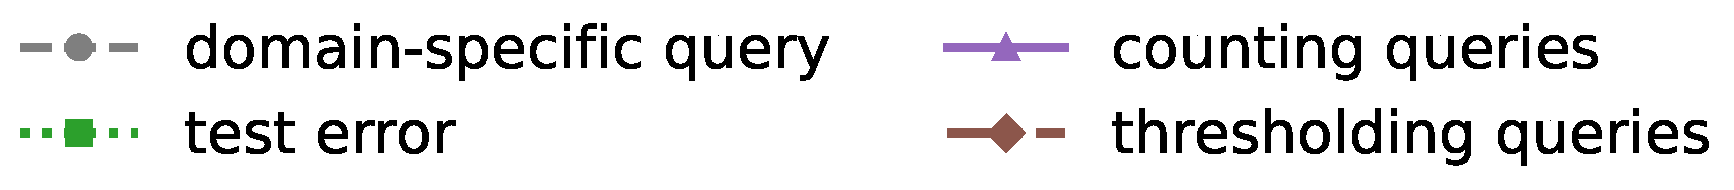
\includegraphics[width=\textwidth]{figures/plots_constraint/exp3_legend.pdf}
    \end{subfigure}
    \begin{subfigure}{.45\linewidth}
        \centering
        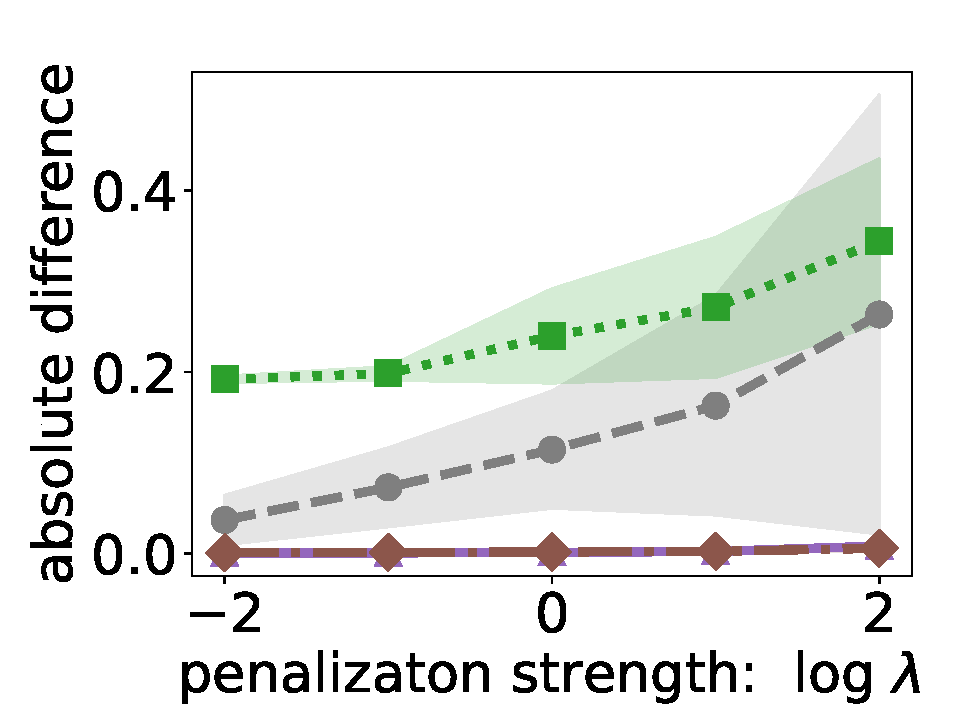
\includegraphics[width=\textwidth]{figures/plots_constraint/exp3_acs_income_CA_2018_default_32+thresholding_1.pdf}
        \caption{ACS Income}
    \end{subfigure}%
    \begin{subfigure}{.45\linewidth}
        \centering
        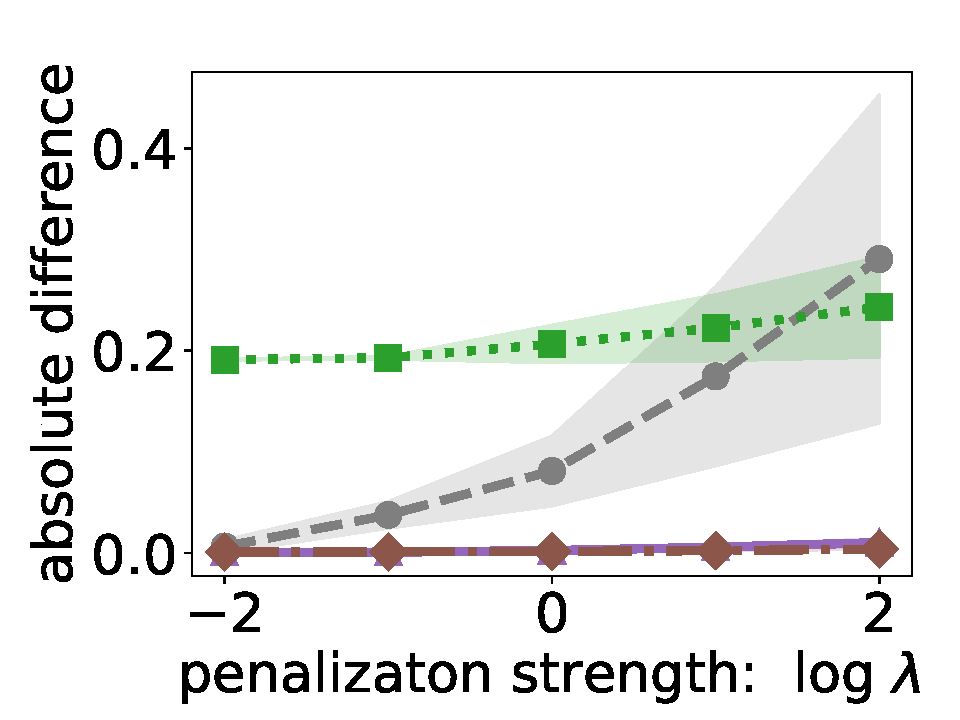
\includegraphics[width=\textwidth]{figures/plots_constraint/exp3_acs_employment_CA_2018_default_32+thresholding_1.pdf}
        \caption{ACS Employment}
    \end{subfigure}
    \caption{\small  The absolute error of the domain-specific query (larger is better), the downstream classification error (smaller is better), and the absolute error over counting and thresholding queries (smaller is better), i.e., only the numerator in ~\Eqref{eq:countquery}, as a function of the log regularization strength $\lambda$. We plot the curves for (a) the Income and (b) the Employment dataset. }
    \label{fig:3}
    \vspace{-0.3in}
\end{wrapfigure}

Section \ref{sec:exp_priv_marginals} shows that PrivPGD constructs a private dataset that successfully preserves the relevant statistics of the original dataset. 
However, while differential privacy protects individual information, many applications require the protection of specific population-level statistics, i.e., one would like specific statistics from the DP-dataset $\dpdata$ to have a large \emph{mismatch} with statistics from the original dataset $D$. 
This goal is in contrast to the utility loss that tries to match certain statistics of the original dataset.
One example is census data, where it might be desirable to hide religious or sexual orientations at the subpopulation level to prevent potential discriminatory misuse of the data. Another example is the publication of rental and house sale prices, where exposing certain correlations could lead to speculative abuses in specific locales.

We now demonstrate how PrivPGD, while constructing a high-quality dataset,
% preserving the metrics from above
 allows the protection of statistics on a population level. As an example, we consider maximizing the distance of a single linear (non-sparse) thresholding query $    \text{thrs}_{\embed}(\particles) = \frac{1}{m} \sum_i 
\mathbbm{1}_{\langle \particles_i, \theta \rangle + b >0}$ defined directly in the embedding space. We approximate this query using a differentiable sigmoid approximation and define $\hat \queryloss(Z) = \frac{1}{c + (\triangle(Z))^2}$ where $\triangle(Z)$ is the difference to a DP-estimate of the original data. We refer to the Appendix~\ref{appendix:details_domain} for details.


 We plot in Figure~\ref{fig:3} the absolute thresholding error as a function of the regularization strength $\lambda$. While the query is well approximated if no (or only little) regularization is used, we see how increasing the regularization strength increasingly protects these statistics, as the domain-specific counting query on $\dpdata$ deviates strongly from the one on the original data $D$. 
We further plot the downstream error and the absolute errors over random counting and thresholding queries (only the numerator in~\Cref{eq:countquery}). We observe that, even for larger regularization penalties, these statistics are still preserved, comparable to the unregularized case. 



\section{Conclusion and future work}


We introduced PrivPGD, a novel generation method for marginal-based private data synthesis. Our approach leverages particle gradient descent, combined with techniques from optimal transport, resulting in improved performance in a large number of settings, enhanced scalability for handling numerous marginals and larger datasets, and increased flexibility for accommodating domain-specific constraints compared to existing methods.

% PrivPGD typically outperforms PGM-based methods and state-of-the-art query-based algorithms like GEM and RAP in our experimental evaluations. However, it is occasionally surpassed by Private GSD. While PrivPGD generally performs better, it is not clear in which specific settings one method outshines the other. 
Future work could develop regularization penalties that promote an inductive bias in PrivPGD towards more favorable solutions, similar to the maximum entropy bias in PGM. Additionally, exploring the design of domain-specific differentiable constraints and applying our method in practical scenarios presents an exciting avenue for future research.


\section{Acknowledgements}

KD was supported by the ETH AI Center and the ETH Foundations of Data Science. JA was supported by the ETH AI Center. We thank Aram Alexandre Pooladin and Guillaume Wang for insightful discussions.





\bibliographystyle{plainnat}
\bibliography{main}
\newpage
\appendix
\section{Extended Experimental Details}
\label{appendix:datasets}
\paragraph{Datasets}
We use a diverse range of real-world datasets, each with associated classification or regression tasks. Notably, our data sources include the American Community Survey (ACS) and various datasets from \cite{grinsztajn2022tree}. 

\begin{itemize}
    \item \textbf{ACS Income classification dataset (Inc.) ~\citep{ding2021retiring}}. The dataset focuses on predicting whether an individual earns more than 50,000 dollars annually. It is derived from the ACS PUMS data sample, with specific filters applied: only individuals aged above 16, those who reported working for at least 1 hour weekly in the past year, and those with a reported income exceeding 100 dollars were included. We take the data from California over a 5-year horizon and survey year 2018, with $d=11$ dimension and $n=760,157$ data points.

    \item \textbf{ACS Employment classification dataset (Emp.)~\citep{ding2021retiring}}. The dataset is designed to predict an individual's employment status. It's derived from the ACS PUMS data sample but only considers individuals aged between 16 and 90. We take the data from California over a 5-year horizon and survey year 2018, with $d=17$ dimension and $n=1,503,938$ data points.
    \item \textbf{ACS Mobility classification dataset (Mob.)~\citep{ding2021retiring}}. The goal is to determine if an individual retained the same residential address from the previous year using a filtered subset of the ACS PUMS data. This subset exclusively includes individuals aged between 18 and 35. Filtering for this age range heightens the prediction challenge, as over 90\% of the broader population typically remains at the same address from one year to the next. We take the data from California over a 5-year horizon and survey year 2018, with $d=22$ dimension and $n=318,332$ data points.
    \item \textbf{ACS Traveltime classification dataset (Tra.)~\citep{ding2021retiring}}. The objective is to predict if an individual's work commute surpasses 20 minutes using a refined subset of the ACS PUMS data. This subset is limited to those who are employed and are older than 16 years. The 20-minute benchmark was selected based on its status as the median travel time to work for the US population in the 2018 ACS PUMS data release. We take the data from California over a 5-year horizon and survey year 2018, with $d=17$ dimension and $n=667,132$ data points.
    \item \textbf{ACS Public Coverage classification dataset (Pub.)~\citep{ding2021retiring}}. The task is to predict if an individual is enrolled in public health insurance using a specific subset of the ACS PUMS data. This subset is narrowed down to individuals younger than 65 and with an income below 30,000 dollars. By focusing on this group, the prediction centers on low-income individuals who don't qualify for Medicare. We take the data from California over a 5-year horizon and survey year 2018, with $d=20$ dimension and $n=583,545$ data points.
    % \item \textbf{Electricity classification~\citep{gama2004learning}}. The Australian New South Wales Electricity Market dataset (ELEC2) reflects the fluctuating prices influenced by demand and supply between 7 May 1996 and 5 December 1998. With $n=30,779$ entries, each representing a 30-minute interval, and $d=7$ features, this dataset provides information on the day, time, and electricity demands of New South Wales and Victoria, and scheduled transfers between these states. The class label indicates the price direction in New South Wales based on the past 24-hour moving average, denoting either an upward or downward trend. Electricity exchanges with Victoria helped stabilize these price shifts.
    % \item \textbf{Diamonds regression~\citep{grinsztajn2022tree}}. The dataset from the tabular benchmark features information on $n=43,152$ diamonds and $d=6$ features. Key attributes include the diamond's price ($326$ to $18,823$), carat ($0.2$ to $5.01$), cut (ranging from Fair to Ideal), color (graded J to D), and clarity (graded I1 to IF). 
    \item \textbf{Medical charges regression dataset (Med.)~\citep{grinsztajn2022tree}}. The dataset from the tabular benchmark, part of the ``regression on numerical features" benchmark, details inpatient discharges under the Medicare fee-for-service scheme. Known as the Inpatient Utilization and Payment Public Use File (Inpatient PUF), it provides insights into utilization, total and Medicare-specific payments, and hospital-specific charges. The dataset encompasses data from over 3,000 U.S. hospitals under the Medicare Inpatient Prospective Payment System (IPPS) framework. Organized by hospitals and the Medicare Severity Diagnosis Related Group (MS-DRG), this dataset spans from Fiscal Year 2011 to 2016. In total, it contains $n=130,452$ data point with $d=3$ features.
    \item \textbf{Black Friday regression dataset (Fri.)~\citep{grinsztajn2022tree}}. This dataset contains purchases from $n=133,456$ buyers on black Friday. Each point is described by $d=9$ features, including gender, age, occupation and marital status.
    % \item \textbf{SGEMM GPU kernel regression~\citep{nugteren2015cltune}}.
    % A  GPU performance data set with  $n=193,280$ points described by discrete vectors with dimension $d=9$.
    % The dataset captures the performance metrics of a matrix multiplication operation, specifically \(A \times B = C\), with matrices of dimensions 2048 x 2048. This computation is executed using an SGEMM GPU kernel (Single Precision General Matrix Multiply) that offers 241600 possible parameter combinations. For each combination, the dataset records the results of 4 separate runs, with the outcomes presented in the final four columns, all measured in milliseconds. The 14 parameters in the set consist of the initial 10 ordinal parameters, which accept up to 4 different powers of two, while the last four parameters are binary. Out of a total of 1,327,104 possible combinations, just 241,600 are viable due to kernel constraints, and this dataset contains outcomes for all feasible combinations. The tests were conducted on a desktop with Ubuntu 16.04, equipped with an Intel Core i5 (3.5GHz), 16GB RAM, and an NVidia Geforce GTX 680 4GB GF580 GTX-1.5GB GPU. The used dataset has $n=193,280$ points described by vectors with dimension $d=9$.
    
    % \item \textbf{Particulate matter air pollution regression~\citep{grinsztajn2022tree}}. The dataset provides hourly readings of particulate matter air pollution in Great Britain for 2017. Commissioned by the UK Department for Environment, Food and Rural Affairs (DEFRA) and the Devolved Administrations, this data is scraped from Ricardo Energy and Environment and made available on the UK AIR website. The dataset contains $n=315,439$ with $d=6$.
    % \item \textbf{Cover type classification~\citep{collobert2001parallel}} Classification of $n=453,281$ pixels into 7 forest cover types based on $d=10$ attributes such as elevation, aspect, slope, hillshade, soil-type, and more.
    \item \textbf{NYC Taxi Green December 2016 regression dataset (Taxi)~\citep{grinsztajn2022tree}}. The dataset, utilized in the ``regression on numerical features" benchmark from the tabular data benchmark, originates from the New York City Taxi and Limousine Commission's (TLC) trip records for the green line in December 2016. In this processed version, string datetime details have been converted to numeric columns. The goal is to predict the ``tip amount". Records exclusively from credit card payments were retained. The dataset contains $n=465,468$ points with $d=9$ features.
    % \item \textbf{Higgs Boson classification~\citep{baldi2014searching}}. The dataset contains $n=752,128$ samples with $d=24$ features. The dataset was generated through Monte Carlo simulations, focusing on kinematic properties measured by particle detectors in accelerators, captured in the first 21 features. The subsequent features are high-level attributes, derived from the initial 21 by physicists, to differentiate between two classes. The goal is to explore deep learning techniques to eliminate the necessity for manual feature creation by physicists. 
    \item \textbf{Diabetes 130-US dataset classification dataset (Diab.)~\citep{strack2014impact}}. The dataset encapsulates a decade (1999-2008) of $n=56,872$ clinical observations from 130 US hospitals and integrated delivery systems, comprising over $d=7$ features denoting patient and hospital results. The data was curated based on specific criteria: the record must be of an inpatient hospital admission, be associated with a diabetes diagnosis, have a stay duration ranging from 1 to 14 days, include laboratory tests, and involve medication administration.
\end{itemize}




\section{Additional Details for Section \ref{sec:domainspecific_exp}}
\label{appendix:details_domain}

We now give additional descriptions for the experiments in Section~\ref{sec:domainspecific_exp}. We approximate the thresholding function  $    \text{thrs}_{\embed}(\particles) = \frac{1}{m} \sum_i 
\mathbbm{1}_{\langle \particles_i, \theta \rangle + b>0}$  using the smooth sigmoid approximation
$
\text{s-thrsh}_{\embed}(\particles) = \frac{1}{m} \sum_i \left(1 + \exp(-\sigma (\langle \theta, \particles_i\rangle-b))\right)^{-1}
$ with $\sigma = 5.0$.  
We then split the privacy budget into two parts; the first part $\epsilon = 0.5$ and $\delta = 2 \times 10^{-6}$ is used for obtaining a DP estimate of 
$\text{s-thrsh}_{\embed}(\embed(D))$ using the Gaussian mechanim, which we denote by $\widehat{ \text{s-thrsh}}_{\embed}$. 
Moreover, we use the remaining privacy budget $\epsilon = 2.0$ and $\delta = 8 \times 10^{-6}$ to privatize all $2$-Way marginals using the Gaussian mechanism as in Algorithm~\ref{alg:mainalgo}. As a result, using the simple composition theorem (see e.g., \cite{dwork2004privacy}), the overall algorithm is then DP for $\epsilon= 2.5$ and $\delta = 10^{-5}$. 

Finally, we generate the differentially private dataset $\dpdata$ by running Algorithm~\ref{alg:pgd} with all privatized 2-Way marginals as inputs as well as the DP regularization loss
\begin{equation}
         \hat \queryloss(\particles) = \frac{0.01}{0.0001 +  ( \text{s-thrsh}_{\embed}(\particles)-\widehat{\text{s-thrsh}}_{\embed})^2}.
     \end{equation}
and regularization strength $\lambda$ reaching from $10^{-2}$ to $10$, as depicted in  Figure~\ref{fig:3}.

\section{Extended Results for Section~\ref{sec:exp_priv_marginals}}
\label{app:extended_results}

We replicate Figure~\ref{fig:comp} with $\epsilon=1.0$ (see Figure~\ref{fig:comp_1}) and $\epsilon=0.2$ (see Figure~\ref{fig:comp_0.2}). At smaller values of $\epsilon$, PrivPGD is more frequently outperformed by PGM, especially in combination with AIM, and also with MST at $\epsilon=0.2$, as well as more often by Private GSD. PGM-based methods benefit from a strong inductive bias towards maximum entropy solutions, which becomes particularly advantageous when noise levels are high. Nevertheless, PrivPGD still maintains highly competitive performance, especially in larger datasets and with fewer features. A similar trend is observed in the total variation and Wasserstein distance, as shown in Figures \ref{fig:comp_sw_tv_1} and \ref{fig:comp_sw_tv_0.2}. These results underscore that PrivPGD's performance edge diminishes as $\epsilon$ decreases. 

Finally, Tables \ref{table_1} to \ref{table_2} provide the detailed metrics for all our results.

 \begin{figure*}[ht!]


    \centering
  \begin{subfigure}{\linewidth}
        \centering

\includegraphics[width=0.9\textwidth]{figures/exp12legend_plot.pdf}
    \end{subfigure}
    \includeBenchFigures{figures/plots_datasets/eps_1.0/}
        \centering
    \caption{\small
    Comparison of PrivPGD with all $2$-way marginals against state-of-the-art methods based on metrics from Section~\ref{subsec:expsetting}: 1) downstream error, 2) covariance error, 3) count. queries error, and 4) thresh. queries error, across 9 tabular datasets. For each method, we plot the $\log_2$ ratio of the errors, using PrivPGD's average error as the denominator, and report the mean and standard deviation over 5 runs. We cut at a log ratio of $y=3$ (dashed line) and list all methods exceeding this threshold above this line in order. We set $\epsilon = 1.0$ and $\delta = 10^{-5}$.}
    
    \label{fig:comp_1}
    \vspace{-0.2in}
\end{figure*}

 \begin{figure*}[ht!]


    \centering
  \begin{subfigure}{\linewidth}
        \centering

\includegraphics[width=0.9\textwidth]{figures/exp12legend_plot.pdf}
    \end{subfigure}
    \includeBenchFigures{figures/plots_datasets/eps_0.2/}
        \centering
 \caption{\small
    Comparison of PrivPGD with all $2$-way marginals against state-of-the-art methods based on metrics from Section~\ref{subsec:expsetting}: 1) downstream error, 2) covariance error, 3) count. queries error, and 4) thresh. queries error, across 9 tabular datasets. For each method, we plot the $\log_2$ ratio of the errors, using PrivPGD's average error as the denominator, and report the mean and standard deviation over 5 runs. We cut at a log ratio of $y=3$ (dashed line) and list all methods exceeding this threshold above this line in order. We set $\epsilon = 0.2$ and $\delta = 10^{-5}$.}
    \label{fig:comp_0.2}
\end{figure*}




\begin{figure*}
    \centering
    \begin{subfigure}{\linewidth}
        \centering
        
\includegraphics[width=0.9\textwidth]{figures/exp12legend_plot.pdf}
    \end{subfigure}
    \includeDistFigures{figures/plots_distances/eps_1.0/}
        \centering
        \caption{\small Comparison of average $\swd_1$ distance (left) and average TV distance (right) for PrivPGD against state-of-the-art methods across 9 tabular datasets. Similar to Figure~\ref{fig:comp}, we report the mean and standard deviation (5 runs) of the $\log_2$ ratio of errors. We set $\epsilon = 1.0$ and $\delta = 10^{-5}$.}

        \label{fig:comp_sw_tv_1}
\end{figure*}

\begin{figure*}
    \centering
    \begin{subfigure}{\linewidth}
        \centering
        
\includegraphics[width=0.9\textwidth]{figures/exp12legend_plot.pdf}
    \end{subfigure}
    \includeDistFigures{figures/plots_distances/eps_0.2/}
        \centering
        \caption{\small Comparison of average $\swd_1$ distance (left) and average TV distance (right) for PrivPGD against state-of-the-art methods across 9 tabular datasets. Similar to Figure~\ref{fig:comp}, we report the mean and standard deviation (5 runs) of the $\log_2$ ratio of errors. We set $\epsilon = 0.2$ and $\delta = 10^{-5}$.}

        \label{fig:comp_sw_tv_0.2}
\end{figure*}




\begin{table*}[ht]
\footnotesize
\centering
\begin{tabular}{cccccccc}
\toprule
dataset & inference & downstream & covariance & counting query & thresholding query & $\swd_1$ distance & TV distance \\
\midrule \multirow{4}{*}{Emp. } & PrivPGD&\textbf{0.19}/0.19 & 0.02 & \textbf{0.00087} & \textbf{0.00043} & \textbf{0.00054} & 0.021 \\
 & PGM+AIM&\textbf{0.19}/0.19 & 0.04 & 0.0025 & 0.0026 & 0.0019 & 0.026 \\
 & PGM+MST&0.33/0.19 & 0.27 & 0.012 & 0.0075 & 0.0087 & 0.1 \\
 & Private GSD&0.2/0.19 & \textbf{0.0083} & 0.0013 & 0.00073 & 0.00059 & \textbf{0.013} \\
\midrule \multirow{6}{*}{Inc. } & PrivPGD&\textbf{0.19}/0.19 & \textbf{0.001} & \textbf{0.00078} & \textbf{0.00031} & \textbf{0.00043} & \textbf{0.028} \\
 & PGM+AIM&\textbf{0.19}/0.19 & 0.014 & 0.0017 & 0.00034 & 0.0017 & 0.034 \\
 & PGM+MST&0.24/0.19 & 0.051 & 0.0077 & 0.0024 & 0.0054 & 0.11 \\
 & Private GSD&0.2/0.19 & 0.0049 & 0.0017 & 0.00083 & 0.00093 & 0.045 \\
 & GEM&0.22/0.19 & 0.047 & 0.01 & 0.0038 & 0.0099 & 0.17 \\
 & RAP&0.2/0.19 & 0.0078 & 0.0017 & 0.00056 & 0.0011 & 0.037 \\
\midrule \multirow{6}{*}{Tra. } & PrivPGD&\textbf{0.37}/0.34 & \textbf{0.0026} & \textbf{0.00065} & \textbf{0.00014} & \textbf{0.00049} & \textbf{0.027} \\
 & PGM+AIM&\textbf{0.37}/0.34 & 0.037 & 0.0023 & 0.00031 & 0.0019 & 0.035 \\
 & PGM+MST&0.46/0.34 & 0.091 & 0.0058 & 0.00032 & 0.0038 & 0.061 \\
 & Private GSD&0.38/0.34 & 0.011 & 0.0017 & 0.00037 & 0.00072 & 0.033 \\
 & GEM&0.4/0.34 & 0.048 & 0.0052 & 0.0011 & 0.0041 & 0.076 \\
 & RAP&0.38/0.34 & 0.015 & 0.0019 & 0.00047 & 0.0014 & 0.036 \\
\midrule \multirow{6}{*}{Pub. } & PrivPGD&\textbf{0.28}/0.27 & 0.06 & \textbf{0.00097} & 0.00033 & 0.00094 & 0.037 \\
 & PGM+AIM&0.32/0.27 & 0.1 & 0.0051 & 0.0012 & 0.0042 & 0.048 \\
 & PGM+MST&0.35/0.27 & 0.41 & 0.01 & 0.00074 & 0.0088 & 0.092 \\
 & Private GSD&0.3/0.27 & \textbf{0.012} & 0.0016 & \textbf{0.00015} & \textbf{0.00057} & \textbf{0.013} \\
 & GEM&0.29/0.27 & 0.035 & 0.0031 & 0.00042 & 0.0019 & 0.029 \\
 & RAP&0.29/0.27 & 0.02 & 0.0015 & 0.00054 & 0.0012 & 0.02 \\
\midrule \multirow{6}{*}{Mob. } & PrivPGD&\textbf{0.23}/0.22 & \textbf{0.0091} & 0.0014 & 0.00051 & 0.0011 & 0.056 \\
 & PGM+AIM&\textbf{0.23}/0.22 & 0.05 & 0.0029 & \textbf{0.00036} & 0.0025 & 0.035 \\
 & PGM+MST&0.24/0.22 & 0.29 & 0.0088 & 0.005 & 0.0095 & 0.096 \\
 & Private GSD&0.24/0.22 & 0.0092 & \textbf{0.0013} & 0.00068 & \textbf{0.00055} & \textbf{0.015} \\
 & GEM&0.24/0.22 & 0.063 & 0.0074 & 0.0022 & 0.006 & 0.082 \\
 & RAP&\textbf{0.23}/0.22 & 0.016 & 0.0014 & 0.00066 & 0.0013 & 0.022 \\
 \bottomrule
 \end{tabular}
 \caption{
    \small The mean of the errors from Section~\ref{subsec:expsetting}  averaged over 5 runs. For the downstream error, we additionally show the test error when training on the original private dataset. We choose $\epsilon =2.5$ and $\delta = 10^{-5}$.}
    \label{table_1}
 \end{table*}
 
 \begin{table*}[ht]
 \footnotesize
\centering
\begin{tabular}{cccccccc}
\toprule
dataset & inference & downstream & covariance & counting query & thresholding query & $\swd_1$ distance & TV distance \\
\midrule \multirow{6}{*}{Taxi } & PrivPGD&\textbf{2.3}/2.2 & \textbf{0.00048} & \textbf{0.00051} & \textbf{0.00011} & \textbf{0.00027} & 0.02 \\
 & PGM+AIM&\textbf{2.3}/2.2 & 0.0013 & 0.00066 & \textbf{0.00011} & 0.0005 & \textbf{0.016} \\
 & PGM+MST&\textbf{2.3}/2.2 & 0.0029 & 0.0011 & 0.0002 & 0.00058 & 0.028 \\
 & Private GSD&\textbf{2.3}/2.2 & 0.004 & 0.0019 & 0.00061 & 0.00093 & 0.064 \\
 & GEM&2.7/2.2 & 0.079 & 0.016 & 0.0037 & 0.018 & 0.36 \\
 & RAP&\textbf{2.3}/2.2 & 0.0065 & 0.0021 & 0.0005 & 0.0013 & 0.078 \\
\midrule \multirow{6}{*}{Fri. } & PrivPGD&\textbf{1.5}/1.4 & \textbf{0.00097} & \textbf{0.00064} & \textbf{0.00053} & \textbf{0.00033} & 0.015 \\
 & PGM+AIM&\textbf{1.5}/1.4 & 0.0014 & \textbf{0.00064} & 0.00058 & 0.00054 & \textbf{0.011} \\
 & PGM+MST&\textbf{1.5}/1.4 & 0.0057 & 0.0027 & 0.0008 & 0.0014 & 0.047 \\
 & Private GSD&1.7/1.4 & 0.0032 & 0.0015 & 0.00083 & 0.0006 & 0.021 \\
 & GEM&2.8/1.4 & 0.031 & 0.0066 & 0.0016 & 0.009 & 0.16 \\
 & RAP&\textbf{1.5}/1.4 & 0.0038 & 0.0018 & 0.00075 & 0.0011 & 0.034 \\
\midrule \multirow{6}{*}{Med. } & PrivPGD&2.2/2.1 & 0.00014 & \textbf{0.0012} & \textbf{0.00013} & \textbf{0.00036} & 0.023 \\
 & PGM+AIM&\textbf{2.1}/2.1 & 0.00066 & \textbf{0.0012} & 0.00034 & 0.00076 & \textbf{0.013} \\
 & PGM+MST&\textbf{2.1}/2.1 & 0.00061 & \textbf{0.0012} & 0.00035 & 0.0007 & 0.017 \\
 & Private GSD&2.2/2.1 & \textbf{0.00013} & \textbf{0.0012} & 0.00014 & 0.00076 & 0.02 \\
 & GEM&75/2.1 & 0.11 & 0.1 & 0.054 & 0.22 & 1.4 \\
 & RAP&4.5/2.1 & 0.0048 & 0.013 & 0.0023 & 0.007 & 0.062 \\
 \midrule
\multirow{6}{*}{Diab. }  & PrivPGD&\textbf{0.4}/0.4 & \textbf{0.0013} & \textbf{0.0013} & 0.00042 & 0.00084 & 0.028 \\
 & PGM+AIM&\textbf{0.4}/0.4 & 0.0045 & 0.0025 & 0.0015 & 0.0022 & 0.028 \\
 & PGM+MST&0.41/0.4 & 0.0047 & 0.0083 & 0.00029 & 0.0017 & 0.045 \\
 & Private GSD&0.41/0.4 & 0.0017 & 0.0017 & \textbf{0.00026} & \textbf{0.00067} & \textbf{0.026} \\
 & GEM&0.41/0.4 & 0.042 & 0.032 & 0.0084 & 0.032 & 0.23 \\
 & RAP&0.41/0.4 & 0.0034 & 0.0021 & 0.00097 & 0.0025 & 0.041 \\
\bottomrule
\end{tabular}
\caption{
    \small The mean of the errors from Section~\ref{subsec:expsetting}  averaged over 5 runs. For the downstream error, we additionally show the test error when training on the original private dataset. We choose $\epsilon =2.5$ and $\delta = 10^{-5}$.}
    \end{table*}




\begin{table*}[ht]
\footnotesize
\centering
\begin{tabular}{cccccccc}
\toprule
dataset & inference & downstream & covariance & counting query & thresholding query & $\swd_1$ distance & TV distance \\

\midrule \multirow{4}{*}{Emp. } & PrivPGD&\textbf{0.19}/0.19 & \textbf{0.0056} & \textbf{0.00077} & \textbf{0.00038} & 0.0006 & 0.027 \\
 & PGM+AIM&0.2/0.19 & 0.063 & 0.0036 & 0.004 & 0.0042 & 0.057 \\
 & PGM+MST&0.23/0.19 & 0.48 & 0.098 & 0.081 & 0.14 & 0.7 \\
 & Private GSD&0.2/0.19 & 0.008 & 0.0014 & 0.00076 & \textbf{0.00059} & \textbf{0.013} \\
\midrule \multirow{6}{*}{Inc. } & PrivPGD&\textbf{0.19}/0.19 & \textbf{0.0019} & \textbf{0.00092} & \textbf{0.00039} & \textbf{0.0006} & 0.042 \\
 & PGM+AIM&\textbf{0.19}/0.19 & 0.014 & 0.0015 & 0.00042 & 0.0016 & \textbf{0.033} \\
 & PGM+MST&0.24/0.19 & 0.052 & 0.0077 & 0.0024 & 0.0054 & 0.11 \\
 & Private GSD&0.2/0.19 & 0.0061 & 0.0017 & 0.00089 & 0.00095 & 0.046 \\
 & GEM&0.22/0.19 & 0.047 & 0.01 & 0.0037 & 0.0098 & 0.16 \\
 & RAP&\textbf{0.19}/0.19 & 0.0074 & 0.0017 & 0.00054 & 0.001 & 0.041 \\
\midrule \multirow{6}{*}{Tra. } & PrivPGD&\textbf{0.37}/0.34 & \textbf{0.0055} & \textbf{0.0011} & 0.00032 & 0.00091 & 0.05 \\
 & PGM+AIM&\textbf{0.37}/0.34 & 0.036 & 0.0027 & 0.00033 & 0.0022 & 0.042 \\
 & PGM+MST&0.44/0.34 & 0.073 & 0.0058 & \textbf{0.00017} & 0.0031 & 0.055 \\
 & Private GSD&0.38/0.34 & 0.011 & 0.0017 & 0.00028 & \textbf{0.00072} & \textbf{0.033} \\
 & GEM&0.4/0.34 & 0.048 & 0.0051 & 0.00091 & 0.004 & 0.074 \\
 & RAP&0.38/0.34 & 0.016 & 0.0019 & 0.0005 & 0.0016 & 0.041 \\
\midrule \multirow{6}{*}{Pub. } & PrivPGD&\textbf{0.28}/0.27 & \textbf{0.011} & 0.0015 & 0.00061 & 0.0014 & 0.061 \\
 & PGM+AIM&\textbf{0.28}/0.27 & 0.058 & 0.0024 & 0.00041 & 0.0023 & 0.028 \\
 & PGM+MST&0.35/0.27 & 0.29 & 0.024 & 0.0092 & 0.04 & 0.21 \\
 & Private GSD&0.29/0.27 & 0.012 & \textbf{0.0014} & \textbf{0.00012} & \textbf{0.00055} & \textbf{0.013} \\
 & GEM&0.29/0.27 & 0.031 & 0.0029 & 0.00056 & 0.0017 & 0.025 \\
 & RAP&0.29/0.27 & 0.022 & 0.0018 & 0.00055 & 0.0014 & 0.023 \\
\midrule \multirow{6}{*}{Mob. } & PrivPGD&\textbf{0.23}/0.22 & 0.021 & 0.0029 & 0.00085 & 0.0026 & 0.13 \\
 & PGM+AIM&\textbf{0.23}/0.22 & 0.054 & 0.0028 & 0.00051 & 0.0024 & 0.034 \\
 & PGM+MST&0.24/0.22 & 0.13 & 0.0077 & 0.0027 & 0.013 & 0.093 \\
 & Private GSD&0.24/0.22 & \textbf{0.0096} & \textbf{0.0012} & \textbf{0.00049} & \textbf{0.0006} & \textbf{0.016} \\
 & GEM&0.24/0.22 & 0.062 & 0.0077 & 0.0021 & 0.0062 & 0.083 \\
 & RAP&\textbf{0.23}/0.22 & 0.021 & 0.0018 & 0.00066 & 0.0017 & 0.031 \\

 \bottomrule
\end{tabular}
\caption{
    \small The mean of the errors from Section~\ref{subsec:expsetting}  averaged over 5 runs. For the downstream error, we additionally show the test error when training on the original private dataset. We choose $\epsilon =1.0$ and $\delta = 10^{-5}$.}
\end{table*}


\begin{table*}[ht]
\footnotesize
\centering
\begin{tabular}{cccccccc}
\toprule
dataset & inference & downstream & covariance & counting query & thresholding query & $\swd_1$ distance & TV distance \\
\midrule \multirow{6}{*}{Taxi } & PrivPGD&\textbf{2.3}/2.2 & \textbf{0.0013} & 0.00077 & 0.00018 & 0.00062 & 0.033 \\
 & PGM+AIM&\textbf{2.3}/2.2 & 0.0014 & \textbf{0.00057} & \textbf{0.00011} & \textbf{0.00046} & \textbf{0.018} \\
 & PGM+MST&\textbf{2.3}/2.2 & 0.003 & 0.0011 & 0.00018 & 0.00055 & 0.029 \\
 & Private GSD&2.4/2.2 & 0.0043 & 0.0018 & 0.00055 & 0.00092 & 0.066 \\
 & GEM&2.8/2.2 & 0.081 & 0.017 & 0.0045 & 0.021 & 0.36 \\
 & RAP&\textbf{2.3}/2.2 & 0.0061 & 0.0021 & 0.00052 & 0.0014 & 0.08 \\
\midrule \multirow{6}{*}{Fri. } & PrivPGD&1.6/1.4 & 0.0022 & 0.00086 & \textbf{0.00053} & 0.00068 & 0.028 \\
 & PGM+AIM&\textbf{1.5}/1.4 & \textbf{0.0016} & \textbf{0.00071} & 0.00056 & \textbf{0.00061} & \textbf{0.014} \\
 & PGM+MST&\textbf{1.5}/1.4 & 0.0058 & 0.0027 & 0.00081 & 0.0015 & 0.049 \\
 & Private GSD&1.6/1.4 & 0.0031 & 0.0015 & 0.00096 & 0.00065 & 0.024 \\
 & GEM&2.8/1.4 & 0.031 & 0.0068 & 0.0014 & 0.0092 & 0.16 \\
 & RAP&1.6/1.4 & 0.0048 & 0.002 & 0.00078 & 0.0016 & 0.046 \\
\midrule \multirow{6}{*}{Med. } & PrivPGD&2.4/2.1 & \textbf{0.00032} & 0.0015 & \textbf{0.00019} & \textbf{0.00061} & 0.03 \\
 & PGM+AIM&2.3/2.1 & 0.00076 & 0.0024 & 0.00053 & 0.00088 & 0.027 \\
 & PGM+MST&\textbf{2.1}/2.1 & 0.00088 & 0.0018 & 0.00051 & 0.001 & 0.023 \\
 & Private GSD&2.2/2.1 & 0.00041 & \textbf{0.0014} & 0.00024 & 0.00095 & \textbf{0.022} \\
 & GEM&75/2.1 & 0.11 & 0.1 & 0.054 & 0.22 & 1.4 \\
 & RAP&4.7/2.1 & 0.0051 & 0.013 & 0.0024 & 0.007 & 0.066 \\
\midrule \multirow{6}{*}{Diab. } & PrivPGD&\textbf{0.4}/0.4 & 0.0033 & 0.0026 & 0.001 & 0.002 & 0.052 \\
 & PGM+AIM&\textbf{0.4}/0.4 & \textbf{0.0031} & \textbf{0.0019} & 0.0014 & \textbf{0.0019} & \textbf{0.03} \\
 & PGM+MST&0.41/0.4 & 0.0042 & 0.0067 & \textbf{0.00056} & \textbf{0.0019} & 0.045 \\
 & Private GSD&0.41/0.4 & 0.0036 & 0.0024 & 0.00096 & 0.0022 & 0.039 \\
 & GEM&0.41/0.4 & 0.04 & 0.031 & 0.0078 & 0.03 & 0.22 \\
 & RAP&0.41/0.4 & 0.0073 & 0.0043 & 0.002 & 0.0054 & 0.071 \\
\bottomrule
\end{tabular}
\caption{
    \small The mean of the errors from Section~\ref{subsec:expsetting}  averaged over 5 runs. For the downstream error, we additionally show the test error when training on the original private dataset. We choose $\epsilon =1.0$ and $\delta = 10^{-5}$.}
    \end{table*}


\begin{table*}[ht]
\footnotesize
\centering
\begin{tabular}{cccccccc}
\toprule
dataset & inference & downstream & covariance & counting query & thresholding query & $\swd_1$ distance & TV distance \\
\midrule \multirow{4}{*}{Emp. } & PrivPGD&\textbf{0.19}/0.19 & 0.015 & 0.0022 & \textbf{0.00078} & 0.0023 & 0.11 \\
 & PGM+AIM&\textbf{0.19}/0.19 & 0.049 & 0.0027 & 0.0031 & 0.0024 & 0.035 \\
 & PGM+MST&0.23/0.19 & 0.1 & 0.0067 & 0.0047 & 0.0043 & 0.05 \\
 & Private GSD&0.2/0.19 & \textbf{0.0088} & \textbf{0.0014} & 0.00083 & \textbf{0.00063} & \textbf{0.014} \\
\midrule \multirow{6}{*}{Inc. } & PrivPGD&\textbf{0.19}/0.19 & 0.0098 & 0.0027 & 0.00086 & 0.0024 & 0.15 \\
 & PGM+AIM&\textbf{0.19}/0.19 & 0.019 & 0.0025 & \textbf{0.00053} & 0.0022 & \textbf{0.048} \\
 & PGM+MST&0.24/0.19 & 0.052 & 0.0077 & 0.0024 & 0.0056 & 0.11 \\
 & Private GSD&0.2/0.19 & \textbf{0.0058} & \textbf{0.0018} & 0.0008 & \textbf{0.001} & 0.052 \\
 & GEM&0.22/0.19 & 0.046 & 0.0099 & 0.0035 & 0.0096 & 0.16 \\
 & RAP&0.2/0.19 & 0.011 & 0.0024 & 0.001 & 0.0019 & 0.072 \\
\midrule \multirow{6}{*}{Tra. } & PrivPGD&0.38/0.34 & 0.027 & 0.0043 & 0.0012 & 0.004 & 0.19 \\
 & PGM+AIM&\textbf{0.37}/0.34 & 0.05 & 0.0028 & 0.00027 & 0.0024 & 0.048 \\
 & PGM+MST&0.44/0.34 & 0.07 & 0.0058 & \textbf{0.00018} & 0.003 & 0.057 \\
 & Private GSD&0.38/0.34 & \textbf{0.012} & \textbf{0.0019} & 0.00033 & \textbf{0.00097} & \textbf{0.041} \\
 & GEM&0.4/0.34 & 0.048 & 0.0051 & 0.00093 & 0.004 & 0.073 \\
 & RAP&0.39/0.34 & 0.026 & 0.003 & 0.00093 & 0.0033 & 0.074 \\
\midrule \multirow{6}{*}{Pub. } & PrivPGD&\textbf{0.29}/0.27 & 0.048 & 0.0058 & 0.0021 & 0.0064 & 0.24 \\
 & PGM+AIM&\textbf{0.29}/0.27 & 0.1 & 0.0039 & 0.00093 & 0.0037 & 0.043 \\
 & PGM+MST&0.31/0.27 & 0.16 & 0.0062 & 0.00031 & 0.0045 & 0.05 \\
 & Private GSD&\textbf{0.29}/0.27 & \textbf{0.014} & \textbf{0.0017} & \textbf{0.0002} & \textbf{0.00085} & \textbf{0.019} \\
 & GEM&\textbf{0.29}/0.27 & 0.044 & 0.0039 & 0.00053 & 0.0025 & 0.035 \\
 & RAP&\textbf{0.29}/0.27 & 0.037 & 0.0033 & 0.0013 & 0.003 & 0.049 \\
\midrule \multirow{6}{*}{Mob. } & PrivPGD&0.24/0.22 & 0.085 & 0.014 & 0.003 & 0.011 & 0.46 \\
 & PGM+AIM&\textbf{0.23}/0.22 & 0.14 & 0.0052 & 0.0019 & 0.0049 & 0.068 \\
 & PGM+MST&0.24/0.22 & 0.12 & 0.006 & 0.0019 & 0.0037 & 0.054 \\
 & Private GSD&0.24/0.22 & \textbf{0.018} & \textbf{0.0019} & \textbf{0.00076} & \textbf{0.0016} & \textbf{0.035} \\
 & GEM&0.24/0.22 & 0.062 & 0.0076 & 0.0018 & 0.0058 & 0.078 \\
 & RAP&0.24/0.22 & 0.048 & 0.0043 & 0.0012 & 0.0048 & 0.08 \\
 \bottomrule
 \end{tabular}
 \caption{
    \small The mean of the errors from Section~\ref{subsec:expsetting}  averaged over 5 runs. For the downstream error, we additionally show the test error when training on the original private dataset. We choose $\epsilon =0.2$ and $\delta = 10^{-5}$.}
    \end{table*}
 
\begin{table*}[ht]
\footnotesize
\centering
\begin{tabular}{cccccccc}
\toprule
dataset & inference & downstream & covariance & counting query & thresholding query & $\swd_1$ distance & TV distance \\
\midrule \multirow{6}{*}{Taxi } & PrivPGD&2.4/2.2 & 0.0055 & 0.0025 & 0.00072 & 0.0026 & 0.11 \\
 & PGM+AIM&\textbf{2.3}/2.2 & 0.0032 & \textbf{0.0011} & 0.00022 & 0.0013 & \textbf{0.037} \\
 & PGM+MST&\textbf{2.3}/2.2 & \textbf{0.003} & 0.0014 & \textbf{0.0002} & \textbf{0.00087} & 0.046 \\
 & Private GSD&2.4/2.2 & 0.0071 & 0.0022 & 0.00068 & 0.0015 & 0.087 \\
 & GEM&2.8/2.2 & 0.082 & 0.017 & 0.0042 & 0.02 & 0.36 \\
 & RAP&2.4/2.2 & 0.011 & 0.0036 & 0.00086 & 0.0036 & 0.17 \\
\midrule \multirow{6}{*}{Fri. } & PrivPGD&2.5/1.4 & 0.011 & 0.0031 & 0.00071 & 0.0031 & 0.11 \\
 & PGM+AIM&\textbf{1.5}/1.4 & \textbf{0.0048} & \textbf{0.0015} & \textbf{0.00061} & \textbf{0.0015} & \textbf{0.036} \\
 & PGM+MST&1.6/1.4 & 0.0069 & 0.003 & 0.00082 & 0.0021 & 0.065 \\
 & Private GSD&1.8/1.4 & 0.0077 & 0.0023 & 0.00088 & 0.0023 & 0.061 \\
 & GEM&2.8/1.4 & 0.031 & 0.0065 & 0.0014 & 0.0083 & 0.15 \\
 & RAP&2.1/1.4 & 0.017 & 0.0042 & 0.001 & 0.0055 & 0.12 \\
\midrule \multirow{6}{*}{Med. } & PrivPGD&3/2.1 & \textbf{0.0013} & \textbf{0.0048} & \textbf{0.00082} & \textbf{0.0024} & 0.076 \\
 & PGM+AIM&3.1/2.1 & 0.0027 & 0.013 & 0.0018 & 0.0033 & 0.12 \\
 & PGM+MST&\textbf{2.2}/2.1 & 0.0026 & 0.0053 & 0.0013 & 0.0031 & \textbf{0.055} \\
 & Private GSD&2.3/2.1 & 0.0028 & 0.0078 & 0.0017 & 0.0067 & 0.056 \\
 & GEM&76/2.1 & 0.11 & 0.1 & 0.054 & 0.21 & 1.4 \\
 & RAP&4.1/2.1 & 0.0084 & 0.018 & 0.0039 & 0.01 & 0.1 \\
\midrule \multirow{6}{*}{Diab. } & PrivPGD&0.42/0.4 & \textbf{0.01} & 0.013 & 0.0045 & 0.0082 & 0.17 \\
 & PGM+AIM&\textbf{0.41}/0.4 & 0.011 & 0.0085 & 0.0042 & \textbf{0.0056} & \textbf{0.071} \\
 & PGM+MST&\textbf{0.41}/0.4 & 0.012 & 0.01 & 0.0044 & 0.008 & 0.1 \\
 & Private GSD&\textbf{0.41}/0.4 & 0.014 & \textbf{0.0083} & \textbf{0.0041} & 0.011 & 0.12 \\
 & GEM&\textbf{0.41}/0.4 & 0.043 & 0.033 & 0.0076 & 0.032 & 0.23 \\
 & RAP&0.42/0.4 & 0.021 & 0.014 & 0.0061 & 0.018 & 0.19 \\
\bottomrule
\end{tabular}
 \caption{
    \small The mean of the errors from Section~\ref{subsec:expsetting}  averaged over 5 runs. For the downstream error, we additionally show the test error when training on the original private dataset. We choose $\epsilon =0.2$ and $\delta = 10^{-5}$.}
    \label{table_2}
    \end{table*}


% \section{Experiments for AP-PGM \citep{mckenna2021relaxed}}
% \label{app:priv_exps}

% Finally,  we compare PrivPGD with AP-PGM \citep{mckenna2021relaxed}. Unlike PrivPGD, AP-PGM does not release a dataset but a regional graph, which allows answering marginal queries (including unseen marginals). Therefore, we evaluate only the average $\swd_1$ and TV distance over all 2-Way marginals. We ran AP-PGM using the official code provided by the authors\footnote{\hyperlink{https://github.com/ryan112358/private-pgm}{https://github.com/ryan112358/private-pgm}} and selected all 2-Way marginals as the workload. We used the Gaussian mechanism for obtaining DP copies of the marginal queries. Table~\ref{tab:your_transposed_label} and Figure~\ref{fig:appgm} show that PrivPGD outperforms AP-PGM on the $\swd_1$ distance, while AP-PGM outperforms PrivPGD on the total variation distance. This outcome is expected, as PrivPGD optimizes the former, while AP-PGM optimizes the latter.




%  \begin{figure*}
%     \centering
%   \begin{subfigure}{\linewidth}
%         \centering
% \includegraphics[width=0.3\textwidth]{aistats/figures/appgm/exp12legend_plot.png}
%     \end{subfigure}
%  \centering
%         \begin{subfigure}{0.32\textwidth}
% \includegraphics[width=\textwidth]{aistats/figures/appgm/0.2.pdf}
%         \caption{$\epsilon = 0.2$}
%     \end{subfigure}
%     \begin{subfigure}{0.32\textwidth}
%         \centering
% \includegraphics[width=\textwidth]{aistats/figures/appgm/1.0.pdf}
%              \caption{$\epsilon = 1.0$}
%         \end{subfigure}
%         \begin{subfigure}{0.32\textwidth}
% \includegraphics[width=\textwidth]{aistats/figures/appgm/2.5.pdf}
%              \caption{$\epsilon = 2.5$}
%     \end{subfigure}
    
%     \caption{
%     \small  Comparison of PrivPGD against AP-PGM, illustrated through the $log_{10}$ ratio of the average $\swd_1$ and TV distances from Section~\ref{subsec:expsetting} averaged over $5$ runs over 15 different tabular datasets as a function of the size of the corresponding datasets. We use different choices for $\epsilon$  and set $\delta = 10^{-5}$. For points above $0$  PrivPGD achieves a smaller error on the corresponding metric, while for points below $0$ the opposite holds. 
% }    
%     \label{fig:appgm}
% \end{figure*}

% \begin{table}[t!]
% \centering
% \begin{tabular}{cccc}
% \toprule
%  Metric &$\epsilon = 0.2$ & $\epsilon = 1.0 $& $\epsilon = 2.5 $\\
% \midrule
%  $\swd_1$  dist. & 10 & 10 & 10 \\
%                                  TV dist.     & 4  & 3  & 2  \\
% \bottomrule
% \end{tabular}
% \caption{Number of times PrivPGD performs better than AP-PGM on the average $\swd_1$ and TV distances from Section~\ref{subsec:expsetting} averaged over $5$ runs evaluated on all 15 different tabular datasets. While PrivPGD wins in most cases for the average $\swd_1$ distance, AP-PGM outperforms PrivPGD on the TV distance.  }
% \label{tab:your_transposed_label}
% \end{table}




\end{document}
